\documentclass[11pt]{article}
\usepackage[margin=1in]{geometry}
\usepackage{amsmath,amssymb,amsthm}
\usepackage{boldtensors}
% boldtensors declares the symbol font `cmbboard' from the bbold family, which
% is not present in every TeX installation (it aborts at the start of math
% mode). Redirect it to the always-available AMS `msb' family; the `"'-syntax
% that would actually render a cmbboard glyph is unused here, so this only
% removes the missing-font dependency.
\DeclareSymbolFont{cmbboard}{U}{msb}{m}{n}
\usepackage{booktabs}
\usepackage{enumitem}
\usepackage{graphicx}
\usepackage{hyperref}

\newcommand{\dd}{\mathrm{d}}
\newcommand{\norm}[1]{\lVert #1 \rVert}
\newcommand{\code}[1]{\texttt{#1}}
\newcommand{\jump}[1]{[\![#1]\!]}
\emergencystretch=3em

\title{Schwarz Coupling for Solid Dynamics in Norma:\\
Transmission Conditions and Interface Energy}
\author{Alejandro Mota}
\date{July--September 2026}

\begin{document}
\maketitle

\begin{abstract}
This note is the reference for the Schwarz transmission conditions
implemented in Norma and for the measurements of their energy behavior in
dynamic solid mechanics. It describes the conditions as they are
implemented now, states the requirements that an energy-consistent
coupling must satisfy, and summarizes the measurements on two benchmarks:
a cantilever beam released from a bent shape, with nonconforming meshes at
a flat interface, and nested cylinders of three materials launched
against a rigid surface, with a closed curved interface. The findings are:
Dirichlet transmission on nonconforming meshes injects energy and ends in
element inversion on both benchmarks; the classical Robin--Robin condition,
which has no absorbing term, does the same, usually sooner, at either of
two Robin parameters; the impedance condition on an overlap boundary is
exact on conforming meshes but cannot be made energy consistent on
nonconforming ones, because the two sides exchange data on two different
surfaces through operators that are not adjoint; and the adjoint-paired
impedance condition on a shared interface, which transfers a single
d'Alembert interface reaction through adjoint operators built from one
cross-mass matrix, never injects energy on either benchmark, is exact at
mild mesh contrast, and dissipates at strong contrast at a rate set by the
part of the interface velocity jump that the two trace spaces cannot
represent in common. The note records the explicit--explicit and
different-time-step variants of that coupling, the behavior of the
relaxation and Aitken acceleration of the Schwarz iteration, and the open
questions, chiefly the stalled interface jump on the cylinders and the
dependence of the converged solution on the Robin parameter.
\end{abstract}

\medskip
\noindent\emph{This document supersedes the July--August 2026 version of
this note and the three earlier notes it consolidated. Measurements that
motivated design decisions but concern superseded variants are kept only
in summary.}

\tableofcontents

\section{Setting}
\label{sec:setting}

\subsection{Decompositions and notation}

A solid body $\Omega \subset \mathbb{R}^3$ is decomposed into two
subdomains $\Omega_1$ and $\Omega_2$ that are integrated independently and
coupled by a Schwarz iteration. The Schwarz framework itself (time
controller, subdomain solves, convergence criteria) follows Mota, Tezaur,
and Phlipot~\cite{MotaTezaurPhlipot2022}, and its contact variant
Mota et al.~\cite{MotaKoliesnikovaTezaurHoy2023}. This note concerns the
transmission conditions imposed on the coupling boundaries and their
energy behavior. Norma supports two geometric configurations.

\paragraph{Nonoverlap.} The subdomains partition $\Omega$ and share an
interface $\Gamma = \partial\Omega_1 \cap \partial\Omega_2$. Let $~n_k$ be
the outward unit normal to $\Omega_k$ on $\Gamma$ (so $~n_1 = -~n_2$) and
$~t_k = ~\sigma_k\,~n_k$ the traction on the side of $\Omega_k$. The
coupled solution must satisfy
\begin{align}
  ~u_1 \;&=\; ~u_2 \qquad \text{(kinematic continuity),}
  \label{eq:continuity} \\
  ~t_1 + ~t_2 \;&=\; ~0 \qquad \text{(traction balance).}
  \label{eq:traction}
\end{align}
The Dirichlet--Neumann method imposes \eqref{eq:continuity} on one side
and \eqref{eq:traction} on the other. The Robin and impedance conditions
of Sec.~\ref{sec:nonoverlap-tc} impose on each side a linear combination
of displacement, velocity, and traction.

\paragraph{Overlap.} The subdomains intersect. Each $\Omega_k$ has a
portion of its boundary, $\Gamma_k \subset \Omega_j$ with $j \ne k$, in the
interior of the partner. That boundary is not shared with $\Omega_j$, so
no mutual traction is directly available there; the partner provides a
well-defined interior state at every point of $\Gamma_k$, and the
conditions of Sec.~\ref{sec:overlap-tc} are built from that state.

Throughout, $~W_k = \int_{\Gamma_k} ~N_k\,~N_k^\top\,\dd\Gamma$ is the
boundary mass matrix of side $k$, $~P$ a kinematic transfer operator that
maps partner data to the interface nodes of a side, the subscript $j$
denotes the partner of side $k$, and $\jump{~q} = ~q_k - ~q_j$ is the
interface jump of a field $~q$, own side minus partner, on the coupling
surface of side $k$. All interface operators are assembled once at
initialization on the reference configuration with the facet Gauss rule
of the receiving side set, and are not updated with the deformation.

\subsection{Vocabulary of the multi-domain controller}
\label{sec:vocabulary}

The controller advances in \emph{stops}. Within a stop each subdomain
advances to the stop end in its own \emph{substeps}, and the
\emph{Schwarz iteration} repeats a \emph{pass} over the subdomains (one
solve of each, with interface data exchanged between them) until the
exchanged data converge; the stop is then committed. The exchanged datum
may be relaxed between Schwarz iterations with a factor
$\theta \in (0, 1]$, fixed or adapted by Aitken extrapolation
(Sec.~\ref{sec:relaxation}). A stop that spans several substeps is a
\emph{window} (Sec.~\ref{sec:windowed}). A mesh pair is \emph{nested} when
every coarse node coincides with a fine node. Mesh ratios are written
$1{:}r$ with $r = h_{\mathrm{fine}}/h_{\mathrm{coarse}}$.

\subsection{Benchmarks}
\label{sec:benchmark}

\paragraph{Cantilever beam.} A linear elastic bar ($E = 6.895$\,GPa,
$\nu = 0.25$, $\rho = 2768$\,kg/m$^3$; $254$\,mm long, $25.4$\,mm tall,
$12.7$\,mm wide) is clamped at one end and released at $t = 0$ from the
parabolic bending displacement $u_y = 0.3937\,x^2$ (tip deflection
$25.4$\,mm), with initial energy $1506$\,J. The subdomain time step is
$1\,\mu$s; horizons are $1$ and $10$\,ms. Subdomain integrators are
trapezoidal Newmark (implicit, I) and central difference (explicit, E),
in the pairings II, IE, EI, and EE (first letter: clamped subdomain).
Overlap decompositions split the bar lengthwise with overlap widths of
$50.8$, $25.4$, and $12.7$\,mm; the nonoverlap decomposition splits it at
$x = 127$\,mm. The free subdomain keeps $h = 6.35$\,mm and the clamped
subdomain is coarsened to $6.35/r$\,mm; the families used are
$r = 1.0, 0.9, \dots, 0.2$ (the mesh-ratio sweep of 2026-07) and
$r \in \{0.9, 0.75, 0.5\}$ (the 2026-09 rerun with the current code and
the Robin--Robin study). The Schwarz iteration is converged to a relative
tolerance of $10^{-8}$ at every stop.

\paragraph{Nested cylinders.} A shell (outer radius $88.9$\,mm, height
$330$\,mm, wall $12.7$\,mm; $E = 200$\,GPa, $\rho = 7823$\,kg/m$^3$)
contains a soft filler (radius $76.2$\,mm, height $305$\,mm; bulk modulus
$5.99$\,GPa, shear modulus $71.7$\,MPa, $\rho = 1843$\,kg/m$^3$) that
contains an offset core (radius $38.1$\,mm, height $102$\,mm, $19$\,mm
above center; $E = 100$\,GPa, $\rho = 4915$\,kg/m$^3$). All three are
neohookean. The P-wave impedance of the filler, $3.35$\,MPa\,s/m, is one
fiftieth of the shell's. The bottom face is fixed in $z$ and the whole
assembly is launched at $-35$\,m/s in $z$, so a compressive front runs
up through the assembly. The decomposition splits the filler at the
boundary of a cylindrical region around the core (radius $57$\,mm, height
$229$\,mm): the interface has a lateral surface and two caps and lies in
one material. The overlap version grows the inner region and shrinks the
outer cavity by $7.6$\,mm each. The inner mesh is $5.1$\,mm and the outer
$6.35$\,mm (ratio $1{:}0.8$, nonconforming), $17$ to $26$ thousand
elements per subdomain; the monolithic reference has $59$ thousand
elements at $5.1$\,mm. Every subdomain uses central difference with
$0.5\,\mu$s stops (Courant number $0.5$) to a horizon of $5$\,ms. One
Cubit journal with a refinement parameter generates all meshes
(\code{examples/jmp/concentric-cylinders}).

\paragraph{Explicit stability.} Central difference in Norma caps its step
at $\mathrm{CFL}\times h_{\min}/c_p$, where $h_{\min}$ is the smallest
element characteristic diameter (twice the mean distance from the element
centroid to its nodes) over the block and $c_p$ the P-wave speed of the
block material; a stop longer than the cap is reached by substeps. On the
cantilever meshes that diameter is about $1.7$ times the edge length, so
the cap at $\mathrm{CFL} = 1$ exceeds the true stability limit; the
cantilever explicit runs at $1\,\mu$s operate at $0.27$ of the measured
limit ($3.6\,\mu$s on the $6.35$\,mm mesh) and are unaffected by it. A
Courant number of $0.5$ or less makes the cap protective on hexahedral
meshes, and the cylinders use $0.5$.

\subsection{Energy metrics}
\label{sec:energy}

\paragraph{Blended energy.} Summing the energies of the two subdomains
counts the overlap region twice, and the double count alone produces
apparent excursions of $\pm 13\%$ as a pulse crosses the overlap. All
energies in this note count the overlap once through a partition of
unity: the production output (\code{blended energy output: true},
\code{src/overlap\_energy.jl}) weights each subdomain by the ratio of its
distance to its own Schwarz boundary to the sum of both distances, a
smooth Arlequin partition, and nonoverlap decompositions receive unit
weights. Results are reported as $E(t)/E(0)$ or as the drift
$E(t)/E(0) - 1$ in percent.

\paragraph{Staggered energy for central difference.} Central difference
conserves, on linear problems, the staggered lumped-mass energy
\begin{equation}
  E_n \;=\; \tfrac12\,\dot{~u}_{n-\frac12}^{T} ~M_L\, \dot{~u}_{n+\frac12}
        + \mathrm{SE}(~u_n)
      \;=\; \tfrac12\,\dot{~u}_n^{T} ~M_L\, \dot{~u}_n
        - \tfrac{\Delta t^2}{8}\, ~a_n^{T} ~M_L\, ~a_n
        + \mathrm{SE}(~u_n),
  \label{eq:staggered}
\end{equation}
with $~M_L$ the lumped mass and $\mathrm{SE}$ the stored energy. The
consistent-mass kinetic energy at integer steps misrepresents the
short-wavelength content of a sharp front: a monodomain central-difference
run of the cantilever reads $-8.2\%$ at $1$\,ms in that metric and
$\pm 0.000\%$ in \eqref{eq:staggered}. Norma's energy output evaluates
\eqref{eq:staggered} for central-difference subdomains, and every
explicit result below uses it. The correction term is negative, so when
grid-frequency content accumulates at the stability limit
($\omega\Delta t \to 2$) the metric goes negative while displacements and
stored energy stay bounded; the note calls that state \emph{bounded and
noisy}.

\section{Transmission conditions on a shared interface}
\label{sec:nonoverlap-tc}

\subsection{Robin coupling}
\label{sec:rr}

On each side of the interface a Robin parameter $\alpha > 0$ is
prescribed and the condition
\begin{equation}
  ~t_k + \alpha\, ~u_k \;=\; ~g_k
    \qquad \text{on } \Gamma, \quad k = 1, 2,
  \label{eq:rr}
\end{equation}
is imposed, with the datum built from the partner's previous Schwarz
iterate, $~g_k^{(n+1)} = -\,~t_j^{(n)} + \alpha\, ~u_j^{(n)}$. At the
fixed point $~u_k = ~u_j$ and $~t_k = -~t_j$, so \eqref{eq:rr} reproduces
\eqref{eq:continuity} and \eqref{eq:traction}. Discretely, the self term
adds the boundary stiffness $\alpha\,~W$ to the tangent and the partner
datum enters the boundary force as
$-~t_j + \alpha\,~W\,~P\,~u_j$. The parameter $\alpha$ has units of
stiffness per unit area (N/m$^3$) and interpolates between a Dirichlet
constraint ($\alpha \to \infty$) and a Neumann condition
($\alpha \to 0$); the classical choice is $\alpha \sim E/h$.

The input keyword is \code{Schwarz RR nonoverlap}. It requires a positive
\code{robin parameter}, rejects \code{impedance scale}, defaults to
\code{adjoint pairing: false} (the classical per-side transfer, which
allows different $\alpha$ on the two sides), and warns when combined with
a dynamic integrator, because the condition reflects every wave
(Sec.~\ref{sec:reflection}) and pumps energy at a dynamic interface
(Secs.~\ref{sec:beam-rr} and \ref{sec:cylinders}). It is intended for
quasi-statics and for comparison studies. Both nonoverlap keywords are
implemented by the same boundary-condition type; the Robin condition is
the $Z = 0$ member of the impedance family, and the two keywords differ
only in defaults and input guards.

\subsection{Impedance coupling}
\label{sec:imp}

For a semi-infinite elastic bar with density $\rho$ and P-wave modulus
$M = \lambda + 2\mu$, an outgoing wave $u(x,t) = f(x - c_p t)$ with
$c_p = \sqrt{M/\rho}$ satisfies
\begin{equation}
  \sigma + Z\,\dot u \;=\; 0,
  \qquad
  Z \;=\; \rho\,c_p \;=\; \sqrt{\rho\,(\lambda + 2\mu)},
  \label{eq:lk}
\end{equation}
the Lysmer--Kuhlemeyer nonreflecting condition~\cite{LysmerKuhlemeyer1969}.
The impedance Schwarz condition adds this absorbing term to
\eqref{eq:rr}:
\begin{equation}
  ~t_k + Z\, \dot{~u}_k + \alpha\, ~u_k \;=\; ~g_k
  \qquad \text{on } \Gamma,
  \qquad
  ~g_k^{(n+1)} \;=\; -\,~t_j^{(n)} + Z\, \dot{~u}_j^{(n)}
     + \alpha\, ~u_j^{(n)}.
  \label{eq:impedance}
\end{equation}
At the fixed point the velocity and displacement terms cancel and
\eqref{eq:impedance} again reproduces continuity and traction balance.
The impedance is computed from the material of the element block that
owns the interface side set, $Z_k = \sqrt{\rho_k(\lambda_k + 2\mu_k)}$,
multiplied by the input \code{impedance scale} (default $1$, required
positive); $\alpha$ is an optional input (default $0$). The keyword is
\code{Schwarz impedance nonoverlap}, with \code{adjoint pairing: true} as
its default (Sec.~\ref{sec:paired}).

Under Newmark integration the end-of-step velocity is linear in the
end-of-step displacement with coefficient $c_v = \gamma/(\beta\,\Delta t)$,
so the self term contributes the tangent $(Z\,c_v + \alpha)\,~W$ and the
self force $~W(Z\,\dot{~u}_k + \alpha\,~u_k)$. In the quasi-static limit
$c_v = 0$ and the condition reduces to \eqref{eq:rr}; a quasi-static run
with $\alpha = 0$ is a pure Neumann condition and does not couple the
subdomains kinematically.

\subsection{Reflection at the interface}
\label{sec:reflection}

Place the interface at $x = 0$ with $\Omega_k$ in $x < 0$ and consider a
harmonic incident wave and its reflection. The Robin condition
$\sigma + \alpha u = 0$ gives the reflection coefficient
\begin{equation}
  R_{\mathrm{RR}}(\omega) \;=\;
     \frac{\mathrm{i}\,\omega\,Z - \alpha}{\mathrm{i}\,\omega\,Z + \alpha},
  \qquad
  \lvert R_{\mathrm{RR}}(\omega) \rvert \equiv 1,
  \label{eq:R-rr}
\end{equation}
so for any real $\alpha > 0$ the interface reflects the incoming wave
completely, with a frequency-dependent phase shift. The impedance
condition $\sigma + Z\dot u + \alpha u = 0$ gives
\begin{equation}
  R_{\mathrm{imp}}(\omega) \;=\;
     -\,\frac{\alpha}{2\,\mathrm{i}\,\omega\,Z + \alpha},
  \qquad
  \lvert R_{\mathrm{imp}}(\omega) \rvert
   = \frac{\alpha}{\sqrt{\alpha^2 + 4\,\omega^2 Z^2}} \;<\; 1,
  \label{eq:R-imp}
\end{equation}
with $R_{\mathrm{imp}} \equiv 0$ at $\alpha = 0$. The dashpot is the only
mechanism in either condition that removes energy from an interface mode;
the Robin spring stores it and returns it.

\section{Transmission conditions on an overlap boundary}
\label{sec:overlap-tc}

\subsection{Dirichlet coupling}
\label{sec:overlap-dbc}

The classical overlap condition imposes the partner's kinematic trace on
$\Gamma_k$,
\begin{equation}
  ~u_k = ~u_j, \qquad \dot{~u}_k = \dot{~u}_j, \qquad \ddot{~u}_k = \ddot{~u}_j
  \qquad \text{on } \Gamma_k,
  \label{eq:overlap-dbc}
\end{equation}
either by pointwise interpolation (locate the partner element that
contains each node in the reference configuration and evaluate the
partner shape functions there) or by the $L^2$ projection
$~P_{kj} = ~W_k^{-1}~L_{kj}$ with
$~L_{kj} = \int_{\Gamma_k} ~N_k\,(~N_j^{\mathrm{vol}})^\top\,\dd\Gamma$.
Both are implemented by \code{SolidMechanicsOverlapSchwarzBoundaryCondition}
(keyword \code{Schwarz overlap}). The constrained degrees of freedom add
no interface tangent.

\subsection{Impedance coupling}
\label{sec:overlap-imp}

The impedance overlap condition leaves the overlap degrees of freedom free
and imposes
\begin{equation}
  ~t_k \,-\, ~t_j
  \;+\; ~Z\,\bigl(\dot{~u}_k - \dot{~u}_j\bigr)
  \;+\; \alpha\,\bigl(~u_k - ~u_j\bigr)
  \;=\; ~0
  \qquad \text{on } \Gamma_k,
  \label{eq:imp-overlap}
\end{equation}
where $~t_j = ~\sigma_j\,~n_k$ is the partner's traction on $\Gamma_k$
with the outward normal of $\Omega_k$ (the partner has no boundary there,
so the converged state satisfies $~t_k = ~t_j$). The own traction $~t_k$
is never computed: it is the natural boundary term of the weak form of
$\Omega_k$, and the condition is imposed by adding the partner datum
$~W(~t_j + ~Z\,\dot{~u}_j + \alpha\,~u_j)$ as a Neumann load and the self
terms $~W(~Z\,\dot{~u}_k + \alpha\,~u_k)$ as an interface force on the
same residual. The impedance is the P/S-split tensor
\begin{equation}
  ~Z \;=\; Z_p\, ~n_k \otimes ~n_k
       \;+\; Z_s\, \bigl(~I - ~n_k \otimes ~n_k\bigr),
  \qquad
  Z_p = \sqrt{\rho(\lambda + 2\mu)}, \quad
  Z_s = \sqrt{\rho\mu},
  \label{eq:imp-tensor}
\end{equation}
with $\rho$, $\lambda$, $\mu$ from the partner's material in the block
named by \code{source block} (each side carries the impedance of its
neighbor, the optimized-Schwarz principle that the transmission operator
should approximate the neighbor's Dirichlet-to-Neumann map). The keyword
is \code{Schwarz impedance overlap}.

\paragraph{The partner traction.} The monodomain solution has continuous
kinematics and a nonzero traction on the artificial surface $\Gamma_k$,
and satisfies \eqref{eq:imp-overlap} identically. Without the term
$-~t_j$ the condition becomes a relative dashpot that the monodomain
solution fails by exactly that traction, and the converged coupled
solution then carries a spurious velocity jump of about $~t/Z$ whose
dissipated power $\lvert ~t \rvert^2/Z$ acts as permanent interface
damping ($59\%$ loss over $1$\,ms on the conforming cantilever;
Sec.~\ref{sec:conforming}). Because $\Gamma_k$ is an interior surface of
the partner mesh, the partner's assembled internal force cannot supply
$~t_j$ there. Norma evaluates it in one of two ways (\code{partner
traction}, default \code{auto}). On node-aligned interfaces the weak
traction is the consistent nodal reaction of the single layer of partner
elements exterior to $\Gamma_k$,
\begin{equation}
  \bigl[ ~W\, ~t_j \bigr]_i
  \;=\; -\sum_{e \,\in\, \mathcal{E}_i^{\mathrm{ext}}}
     \bigl( ~f^{\mathrm{int}}_e + ~M_e\, \ddot{~u}_e \bigr)_i,
  \label{eq:consistent-traction}
\end{equation}
which the monodomain solution satisfies identically, mesh-scale content
included (implemented by
\code{build\_consistent\_traction\_patch!}). Otherwise the
partner's consistently recovered nodal stress is transferred to
$\Gamma_k$ and contracted with the outward normal; recovery is enabled
automatically for models that carry this condition.

\paragraph{Transfer and assembly.} The kinematic fields and the recovered
stress are transferred by the $L^2$ projection by default
(\code{transfer: variational}; pointwise interpolation is a legacy
option, and the two coincide on node-aligned interfaces). On non-aligned
interfaces the whole partner datum is assembled on the partner's offset
surface from the partner's own nodal values and transferred with one
surface-to-surface operator (\code{characteristic\_partner\_terms}). The
self tangent consists of the nodal blocks
$W_{ij}\,(c_v\,~Z(~n_j) + \alpha\,~I)$. A scalar or step-dependent
multiplier on $~Z$ (\code{impedance scale}) remains available; with the
traction term in place the physical scale $1$ is the conserving one, and
the historical use of the scale as a per-problem parameter, which
compensated the missing traction, is obsolete. With
\code{impedance scale: 0} the condition is the Robin--Robin overlap
condition $~t_k - ~t_j + \alpha\,(~u_k - ~u_j) = ~0$; no separate keyword
exists for it.

\subsection{Summary of the four conditions}

\begin{table}[htbp]
\centering
\small
\caption{Transmission conditions on a shared (nonoverlap) interface.}
\label{tab:nonoverlap-conditions}
\begin{tabular}{lcc}
\toprule
& Robin & Impedance \\
\midrule
Boundary condition &
  $~t_k + \alpha\, ~u_k = ~g_k$ &
  $~t_k + Z\, \dot{~u}_k + \alpha\, ~u_k = ~g_k$ \\[0.3em]
Self tangent &
  $\alpha\, ~W$ &
  $(Z\, c_v + \alpha)\, ~W$ \\[0.3em]
Self force &
  $\alpha\, ~W\, ~u_k$ &
  $~W\,\bigl(Z\, \dot{~u}_k + \alpha\, ~u_k\bigr)$ \\[0.3em]
Partner datum &
  $-~t_j + \alpha\, ~W\, ~P\, ~u_j$ &
  $-~t_j + Z\, ~W\, ~P\, \dot{~u}_j + \alpha\, ~W\, ~P\, ~u_j$ \\[0.3em]
$Z$ &
  (none) &
  interface block material; harmonic mean per pair \\[0.3em]
$\alpha$ &
  input, required, per side &
  input, optional, one value per interface \\[0.3em]
Transfer &
  per side (legacy) &
  adjoint pair from one cross-mass matrix \\[0.3em]
Reflection $\lvert R \rvert$ &
  $\equiv 1$ &
  $< 1$; $0$ at $\alpha = 0$ \\[0.3em]
Keyword &
  \code{Schwarz RR nonoverlap} &
  \code{Schwarz impedance nonoverlap} \\
\bottomrule
\end{tabular}
\end{table}

\begin{table}[htbp]
\centering
\footnotesize\setlength{\tabcolsep}{4pt}
\caption{Transmission conditions on an overlap boundary.}
\label{tab:overlap-conditions}
\begin{tabular}{lcc}
\toprule
& Dirichlet & Impedance \\
\midrule
Boundary condition &
  $~u_k = ~u_j$ (pointwise or $L^2$) &
  $~t_k - ~t_j + ~Z\,(\dot{~u}_k - \dot{~u}_j) + \alpha\,(~u_k - ~u_j) = ~0$ \\[0.3em]
Self tangent &
  (DOFs constrained) &
  $W_{ij}\,\bigl(c_v\, ~Z(~n_j) + \alpha\, ~I\bigr)$ \\[0.3em]
Self force &
  (none) &
  $~W\,\bigl(~Z\, \dot{~u}_k + \alpha\, ~u_k\bigr)$ \\[0.3em]
Partner datum &
  $~u_k \leftarrow ~P\, ~u_j$ &
  $~W\,\bigl(~t_j + ~Z\, \dot{~u}_j + \alpha\, ~u_j\bigr)$ \\[0.3em]
Partner traction &
  (none) &
  consistent \eqref{eq:consistent-traction} or recovered stress \\[0.3em]
$~Z$ &
  (none) &
  partner material, P/S split \\[0.3em]
$\alpha$ &
  (none) &
  input, optional \\[0.3em]
Keyword &
  \code{Schwarz overlap} &
  \code{Schwarz impedance overlap} \\
\bottomrule
\end{tabular}
\end{table}

\section{Requirements for energy consistency}
\label{sec:theory}

Three results from the literature fix the structure of an
energy-consistent coupling; the measurements of
Secs.~\ref{sec:beam}--\ref{sec:cylinders} confirm each of them.

\paragraph{The interface work identity.} For Newmark-family subdomains
coupled by interface tractions, the discrete energy balance over a step
contains the interface term
(Gravouil--Combescure~\cite[Eq.~(34)]{GravouilCombescure2001};
Karimi--Nakshatrala~\cite[Eq.~(84)]{KarimiNakshatrala2014})
\begin{equation}
  E_{\mathrm{int}}
  = \sum_{\text{sides }k} \frac{1}{\Delta t_k}\,
    \jump{\dot{~u}_k}^{T} ~C_k^{T}\, \jump{\Lambda_k},
  \label{eq:eint}
\end{equation}
the work of the transmitted tractions through the kinematic jump, each
side on its own grid ($~C_k$ is the interface restriction of side $k$,
$\Lambda_k$ the traction impulse transmitted to it, and $\jump{\cdot}$
here the change across the step). The term vanishes if and only if the
traction is one field acting equal and opposite on the two sides through
adjoint trace operators, with velocity continuity enforced at instants
shared by both time grids. When the pairing is broken the term has no
sign.

\paragraph{Representability on nonconforming grids.} Gander, Halpern,
and Nataf~\cite{GanderHalpernNataf2003} prove convergence of Schwarz
waveform relaxation with impedance transmission on nonmatching grids
under three conditions: Robin-type (not Dirichlet) transmission, a
consistent boundary discretization of the transmission operator, and an
intergrid transfer that is an $L^2$ contraction (a projection qualifies;
pointwise interpolation does not). The choice $Z = \rho c$ is the exact
transparent operator in one dimension. On nonconforming grids the coupled
system defines the converged solution; there is no monodomain scheme it
equals. Continuity holds only through the projection, and the component
of the fine trace orthogonal to the coarse trace space is never matched:
the dashpot then absorbs that persistent component as an absorbing
boundary would, which is sign-definite dissipation, required for
stability. Achdou, Japhet, Maday, and Nataf~\cite{AchdouJaphetMadayNataf2002}
locate the remedy in a common trace space for the datum, not in a better
$Z$.

\paragraph{The adjoint requirement.} Energy-stable discontinuous Galerkin
couplings~\cite{AppeloWang2019,DuruEtAl2021,LiuEtAl2023} compute one
interface state on a common description of the interface and use it in
both weak forms; the interface power then reduces to
\begin{equation}
  P \;=\; -\int_\Gamma \jump{\dot{~u}}^T ~Z \jump{\dot{~u}} \,\dd S
  \;\le\; 0,
  \label{eq:telescope}
\end{equation}
which is confined to the jump and vanishes under refinement and at
convergence. The discrete requirement is that the two kinematic transfers
be $L^2$-adjoint through one cross-mass matrix,
\begin{equation}
  ~W_1 \Pi_{2\to1} \;=\; \bigl(~W_2\,\Pi_{1\to2}\bigr)^{T} \;=\; ~B,
  \qquad
  B_{mn} = \int_\Gamma \varphi^1_m\,\varphi^2_n \,\dd S .
  \label{eq:adjoint}
\end{equation}
Two independent interpolations violate \eqref{eq:adjoint}, the cross
terms of the interface power do not cancel, and its sign is undetermined.
Liu et al.~\cite{LiuEtAl2023} add that interface unknowns may need
implicit treatment even between explicit interiors.

\paragraph{Consequence for the two decompositions.} Condition
\eqref{eq:adjoint} presumes one shared surface on which the two works
cancel. The overlap decomposition has none: data are exchanged on two
distinct surfaces $\Gamma_1$ and $\Gamma_2$, so no pairing of the two
works exists, and energy consistency could only come from agreement of
the two discrete solutions in the overlap, which the differing discrete
dispersion relations of the two grids preclude at fixed $h$
(Sec.~\ref{sec:overlap-remedies}). The nonoverlap decomposition has a
shared interface, and the adjoint-paired coupling of
Sec.~\ref{sec:paired} implements \eqref{eq:adjoint} on it.

\section{The adjoint-paired nonoverlap impedance coupling}
\label{sec:paired}

This section describes the coupling as implemented (the default of
\code{Schwarz impedance nonoverlap}; \code{adjoint pairing: false}
restores the legacy per-side transfer). Its measured behavior is in
Secs.~\ref{sec:beam-nonoverlap} and \ref{sec:cylinders}.

\subsection{Construction}
\label{sec:paired-construction}

\paragraph{Transfer operators.} The cross-mass matrix $~B$ of
\eqref{eq:adjoint} is integrated over the facets of the finer side (the
side with more interface nodes): each facet quadrature point is mapped to
the partner surface by closest-point projection in the reference
configuration and the partner facet shape functions are evaluated there.
This rule is exact when the coarser trace mesh is nested in the finer
facets and carries facet-quadrature error where a coarse basis function
kinks inside a fine facet; the partition-of-unity error
$\max_i \lvert (\Pi_k \mathbf{1} - \mathbf{1})_i \rvert$ is logged at
setup as a certificate (zero on conforming and nested interfaces). The
kinematic transfers are $\Pi_1 = ~W_1^{-1}~B$ and
$\Pi_2 = ~W_2^{-1}~B^{T}$, the force transfers their partner adjoints
$N_1 = \Pi_2^{T}$ and $N_2 = \Pi_1^{T}$, all scalar and applied to each
Cartesian component.

\paragraph{Exchanged traction.} The weak partner reaction of side $j$ is
the restriction to its interface degrees of freedom of its assembled
d'Alembert residual,
\begin{equation}
  \lambda_j \;=\; -\bigl(~M_j\,\ddot{~u}_j + ~f^{\mathrm{int}}_j
   - ~f^{\mathrm{body}}_j\bigr)\big|_{\Gamma},
  \label{eq:dalembert}
\end{equation}
with $~M_j$ the mass matrix its integrator uses (consistent for Newmark,
lumped for central difference). With this reaction the two interface rows
sum exactly to the monodomain row, so the monodomain trajectory is the
fixed point. The legacy coupling transferred the static reaction
$-~f^{\mathrm{int}}$; in dynamics the two sides' static reactions differ
by the inertia of the interface nodes, each side carrying its own
tributary mass, and the fixed point then differs from the monodomain
discretization by a steady, step-independent interface energy loss
($-9.6\%$ per millisecond on the conforming cantilever, Table~\ref{tab:legacy-paired}).

\paragraph{Pair impedance and Robin parameter.} The pair shares one
impedance, the harmonic mean $2Z_1 Z_2/(Z_1 + Z_2)$ of the per-side
material impedances $Z_k = \rho_k c_{p,k}$ of the blocks that own the
two side sets, each multiplied by its side's \code{impedance scale}; this
is the Riemann-solver weighting of~\cite{DuruEtAl2021,LiuEtAl2023}. The
Robin parameter $\alpha$ is one value per interface: the spring stores
and returns energy conservatively only when both interface forces pair
through the same coefficient, so mismatched values abort with a message
naming both side sets. The pair impedance is scalar (P-wave); a tensor
pair impedance has not been needed on the benchmarks studied.

\paragraph{Partner datum.} Side $k$ receives
\begin{equation}
  ~g_k \;=\; N_k\,\lambda_j
   \;+\; Z\,~B_k\,\dot{~u}_j
   \;+\; \alpha\,~B_k\,~u_j,
  \qquad ~B_1 = ~B,\quad ~B_2 = ~B^{T},
  \label{eq:paired-rhs}
\end{equation}
with the partner fields evaluated at side $k$'s current substep time
(Sec.~\ref{sec:subcycle}). The self terms, the tangent
$(Z c_v + \alpha)\,~W_k$ and the force
$~W_k(Z\,\dot{~u}_k + \alpha\,~u_k)$, are assembled with the internal
force at every residual evaluation.

\paragraph{What the parameters change.} At the fixed point the two
conditions add to traction balance and subtract to
$Z\,\dot{~\delta} + \alpha\,~\delta = ~0$ for the interface jump
$~\delta$. When the jump can close, as it does on conforming and nested
meshes, the converged solution is independent of $Z > 0$ and
$\alpha \ge 0$, and both act only on the convergence rate of the
iteration. On nonconforming meshes the jump closes only in the projected
sense of \eqref{eq:adjoint} and the accepted iterate has a residual
jump, so the $\alpha$ term is a spring force on that residual, and its
influence on the converged coupled solution has not been measured for
the paired coupling (Sec.~\ref{sec:open}). The classical Robin--Robin
runs of Sec.~\ref{sec:beam-rr} show that with per-side transfer the
converged solution does depend on $\alpha$.

\subsection{Explicit subdomains}
\label{sec:imex}

With a central-difference subdomain on either side, the coupling is
strongly unstable if the interface terms are evaluated at lagged time
levels: the exchanged reaction \eqref{eq:dalembert} couples the partner's
acceleration into the interface force, an algebraic loop that the
implicit pairs resolve within the Newton iteration. Following Liu et
al.~\cite{LiuEtAl2023}, the explicit update is closed implicitly on the
interface rows only,
\begin{equation}
  \bigl(~M + \gamma\,\Delta t\,Z\,~W\bigr)\big|_\Gamma\, ~a_{n+1}
  \;=\; ~M\,~a^{\mathrm{expl}}\big|_\Gamma,
  \label{eq:imex}
\end{equation}
a small symmetric positive definite solve per interface, factored once
and reused for the three components while the operator is unchanged
(\code{imex\_interface\_acceleration!}); the interior stays explicit.
Here $~M\big|_\Gamma$ is the lumped mass on the interface rows, $~W$ the
side's own boundary mass matrix, $\gamma = \tfrac12$, and
$~a^{\mathrm{expl}}$ the plain explicit update, whose right-hand side
contains the dashpot at the predictor velocity and the Robin spring at
the known end-of-step displacement; the solve replaces the
predictor-velocity dashpot by the end-of-step one. The Robin spring
stays explicit, so a large $\alpha$ can violate the central-difference
stability limit on the interface rows. Interface degrees of freedom held
by Dirichlet conditions keep their prescribed acceleration and enter the
free rows as data.

\subsection{Different time steps per subdomain}
\label{sec:subcycle}

Each subdomain records full-field snapshots (displacement, velocity,
acceleration, assembled internal force) at every substep of every
Schwarz iteration, anchored by a snapshot of the stop-start state. When a
coupling condition is evaluated at time $t$, each field is interpolated
piecewise linearly to $t$ (queries beyond the history clamp to its
endpoints), the partner state is temporarily replaced by the
interpolants, the coupling terms are evaluated, so the reaction
\eqref{eq:dalembert} is formed from the interpolated acceleration and
internal force, and the partner state is restored. This is the
interpolated-continuity structure under which Gravouil and
Combescure~\cite{GravouilCombescure2001} prove the interface work of the
subcycled exchange nonpositive and of order $\Delta t$. Two earlier
defects (an off-by-one in the segment selection and a missing stop-start
anchor) had reduced the exchange to end-sampled constant data; both are
fixed and the measurements below use the interpolated exchange.

Three constructions that would make the coarse side's datum exactly
work-conjugate to the fine side's interpolation, as in Prakash and
Hjelmstad~\cite{PrakashHjelmstad2004}, were implemented and all fail in
a partitioned exchange: the trapezoidal window average lags the
interface motion by half a window and adds dissipation; the recursion
$\hat\lambda_{n+1} = 2\overline{\lambda} - \hat\lambda_n$ doubles the
contraction factor of the Schwarz iteration and diverges within tens of
stops; and the least-squares endpoint fit is an extrapolation whose gain
exceeds one outside the linear band and injects energy without bound
over hundreds of stops. Only causal transfer operators are robust in a
fixed-point exchange; exact cancellation of the subcycled interface work
requires a direct interface solve, as Prakash and Hjelmstad use. The
window-average and endpoint-fit utilities remain in
\code{interpolation.jl} as tested building blocks.

\subsection{Relaxation and Aitken acceleration}
\label{sec:relaxation}

The relaxed datum is the assembled $~g_k$ of \eqref{eq:paired-rhs} on
one side of each pair (the later-listed subdomain); a fresh relaxation
slot starts from zero rather than from the incoming datum. Two Aitken
forms are available (\code{relaxation: aitken recursive} and
\code{aitken secant}), with \code{relaxation parameter} the fixed or
initial factor and \code{aitken N0 parameter} the number of initial
Schwarz iterations at the input factor.

\paragraph{State keyed by substep slot.} The relaxation state (the
stored datum and the Aitken residuals) is keyed per pair and per substep
time slot within the stop, and cleared at every stop
(\code{relaxation\_slot!}). Before this, one vector per pair was updated
at every application of the condition, so a stop spanning several
substeps blended iterates across time, a causal low-pass filter on the
exchanged traction that shifted the fixed point (measured on the
conforming cantilever at $10$\,ms: $+11\%$ to $-84\%$ with Aitken and
$-7\%$ to $-88\%$ with fixed $\theta = 0.5$ as the window grew from $2$
to $10$ substeps). With the slot-keyed state, windowed stops
reproduce the same-step trajectory to Schwarz truncation
(Sec.~\ref{sec:windowed}).

\paragraph{Guards.} On the Dirichlet-transfer paths (overlap and
Dirichlet--Neumann) a fresh slot seeds the stored iterate with the
incoming datum, so the first residual is exactly zero and the secant
factor evaluates to $-0.0$; a zero factor freezes the interface, and in a
chain of three or more subdomains the whole Schwarz iteration then
reports convergence after one iteration with an answer wrong by $100\%$.
The secant update is now taken only when the residual difference exceeds
a floor, a factor of magnitude below $10^{-12}$ is recorded on the
controller, and the convergence criterion refuses to accept that
iteration. The recursive form no longer runs the first \code{N0}
iterations unrelaxed regardless of the input factor.

\paragraph{Where Aitken applies.} Aitken acceleration is applied only to
single-slot stops (\code{aitken\_applies}); in windowed stops the
residuals of different slots belong to different times and the
extrapolated factor overshoots. On the implicit cantilever pairs it
reduces the Schwarz iterations by about a factor of ten against a fixed
factor of $0.5$ ($599$ against $56$ recursive or $58$ secant over ten
stops). On the explicit cylinders pair (Sec.~\ref{sec:cylinders}) every
Aitken form diverges: the displacement residual between successive
iterations collapses while the interface velocity jump stalls at a finite
value, the extrapolated factor exceeds $2$ by the second or third
iteration, oscillates between $-10$ and $+3$, and the iteration reaches
the cap of $256$ within the first $25$ stops, after which an element
inverts; the recursive form with \code{N0} $= 2$ and the secant form fail
the same way, six stops later. A fixed factor of $0.5$ converges there in
$2$ to $3$ iterations per stop, and $\theta = 1$ (no relaxation) diverges
after $0.3$\,ms.

\section{Measurements on the cantilever beam}
\label{sec:beam}

\subsection{Overlap, conforming meshes: the partner traction}
\label{sec:conforming}

On the conforming node-aligned overlap pair (II, $\alpha = 0$, physical
impedance) the energy error of the impedance overlap coupling over
$1$\,ms decreases through four corrections, none with a parameter:
\[
  \underbrace{59\%}_{\text{no partner traction}}
  \;\longrightarrow\;
  \underbrace{14\%}_{\text{traction from lumped recovery}}
  \;\longrightarrow\;
  \underbrace{1.5\%}_{\text{consistent recovery}}
  \;\longrightarrow\;
  \underbrace{0.08\%}_{\text{consistent traction \eqref{eq:consistent-traction}}}
\]
against the $0.1\%$ of converged conforming Dirichlet coupling. The
residual of the recovered-stress step was diagnosed with an
interface-work instrumentation that separates the partner-traction,
dashpot, and Robin channels (\code{report\_impedance\_interface\_work},
environment-gated, CSV through \code{NORMA\_IMPEDANCE\_WORK\_CSV}): it is
unchanged under a Schwarz tolerance of $10^{-11}$ and under halving the
time step, and it halves when $h$ is halved. The recovery error on
mesh-scale content is converted by the transmission condition into a
velocity jump of about $\delta t/Z$ that the dashpot dissipates at rate
$\lvert \delta t \rvert^2/Z$ over the whole run; the consistent traction
removes it (integrated dashpot work $-42.6$\,J $\to$ $+0.1$\,J). The
P/S tensor impedance \eqref{eq:imp-tensor}, which appeared worse than a
scalar one with recovered stress ($4.1\%$ against $1.5\%$), is exact with
the consistent traction ($0.076\%$): its smaller shear impedance
amplified the tangential recovery error. Historical per-problem tuning
of the impedance scale, whose best value on the nonconforming pair was
$1.12$, compensated the missing traction against transfer injection and
is obsolete.

\subsection{Overlap, nonconforming meshes: sign-indefinite interface work}
\label{sec:overlap-nonconforming}

Table~\ref{tab:ratio-sweep} gives the drift at $1$\,ms of the impedance
overlap coupling with variational transfer across nine mesh ratios,
three overlap widths, and four integrator pairings ($108$ runs).

\begin{table}[htbp]
\centering
\small\setlength{\tabcolsep}{3.6pt}
\caption{Energy drift at 1\,ms of the impedance overlap coupling
(variational transfer, blended energy), in percent.}
\label{tab:ratio-sweep}
\begin{tabular}{l rrrr rrrr rrrr}
\toprule
& \multicolumn{4}{c}{overlap 50.8\,mm} & \multicolumn{4}{c}{overlap 25.4\,mm}
& \multicolumn{4}{c}{overlap 12.7\,mm} \\
\cmidrule(lr){2-5}\cmidrule(lr){6-9}\cmidrule(lr){10-13}
ratio & II & IE & EI & EE & II & IE & EI & EE & II & IE & EI & EE \\
\midrule
1:1.0 & $-0.1$ & $-8.9$ & $-0.2$ & $+8.7$ & $-0.1$ & $+5.0$ & $-0.4$ & $+10.2$ & $-0.0$ & $-15.7$ & $-6.1$ & $+3.6$ \\
1:0.9 & $+7.6$ & $-11.7$ & $-5.5$ & $+8.5$ & $-4.4$ & $-8.1$ & $+4.4$ & $+9.1$ & $+0.1$ & $-14.8$ & $-1.0$ & $+4.3$ \\
1:0.8 & $\mathbf{+29.8}$ & $-15.3$ & $+5.5$ & $-9.5$ & $+20.4$ & $\mathbf{+45.1}$ & $-2.4$ & $-1.9$ & $-3.1$ & $-20.3$ & $-5.4$ & $+4.7$ \\
1:0.7 & $+19.2$ & $-12.8$ & $+2.7$ & $-11.6$ & $+11.8$ & $-18.6$ & $+0.7$ & $-5.4$ & $+11.1$ & $+7.3$ & $-9.8$ & $-17.9$ \\
1:0.6 & $-61.1$ & $-54.0$ & $-57.7$ & $-40.4$ & $+2.1$ & $-18.6$ & $-63.9$ & $-53.4$ & $-4.5$ & $-34.2$ & $-57.1$ & $-52.7$ \\
1:0.5 & $-50.6$ & $-32.3$ & $-36.4$ & $-56.8$ & $-11.0$ & $-17.6$ & $-55.7$ & $-54.3$ & $-29.2$ & $-54.0$ & $-56.8$ & $-52.0$ \\
1:0.4 & $-12.4$ & $+3.9$ & $-43.1$ & $-53.1$ & $-52.7$ & $-50.2$ & $-57.0$ & $-63.8$ & $-36.6$ & $-52.4$ & $-78.2$ & $-76.2$ \\
1:0.3 & $-65.0$ & $-44.5$ & $-78.3$ & $-57.4$ & $\mathbf{+173.7}$ & $\mathbf{+274.7}$ & $-81.2$ & $-78.8$ & $-30.5$ & $-58.6$ & $-79.5$ & $-79.4$ \\
1:0.2 & $-79.1$ & $-76.8$ & $-80.8$ & $-78.9$ & $-66.5$ & $-66.2$ & $-86.3$ & $-87.4$ & $-22.2$ & $-45.8$ & $-91.2$ & $-90.3$ \\
\bottomrule
\end{tabular}
\end{table}

Conforming implicit runs conserve to $0.1\%$ at every width. Every
nonconforming configuration either loses tens of percent or gains: the II
column injects at mild coarsening at nearly every width (up to $+29.8\%$
at $1{:}0.8$), the $25.4$\,mm IE run at $1{:}0.3$ reaches $+275\%$, and
the drift is not monotone in the ratio (at $25.4$\,mm the II column moves
$-52.7 \to +173.7 \to -66.5\%$ across $1{:}0.4$, $1{:}0.3$, $1{:}0.2$). The
sign of the interface work is decided by the mesh pair and the overlap
geometry together, and no a priori bound on its sign or magnitude
exists. The channel instrumentation shows the mechanism: on the
$50.8$\,mm/$1{:}0.5$ II case with pointwise transfer the dashpot does
$+554$\,J of positive work over $1$\,ms, which a dissipator cannot do, so
the discrete dashpot term is not a quadratic form; the two sides
interpolate partner fields with unrelated operators and their dashpot
terms do not pair.

\paragraph{Dirichlet control.} The same nine mesh configurations with
Dirichlet overlap coupling (II) conserve to $\pm 0.05\%$ on conforming
meshes and are severely unstable on every nonconforming one ($+22\%$ to
$+7765\%$ at $1$\,ms, most runs ending in Newton divergence before
$1$\,ms), with pointwise and with weak transfer alike. The dashpot of the
impedance condition is therefore what stabilizes a coupling that
kinematic matching destabilizes, and its dissipation is the energy of
the inter-grid discrepancy it absorbs.

\paragraph{Ten milliseconds.} Of the $108$ overlap runs rerun to $10$\,ms,
$74$ ended by element inversion after exponential energy growth
(typically $30$ to $100$ times $E(0)$ at failure, between $2$ and $9$\,ms)
and most of the remainder decayed toward zero energy. Configurations that
appeared dissipative at $1$\,ms reversed and grew. Conformity does not
stabilize the mixed pairings: the conforming $25.4$\,mm IE run grew
exponentially and failed at $6.25$\,ms. The only overlap configurations
stable and accurate at $10$\,ms are the conforming II runs ($+0.6$,
$+0.6$, $+0.2\%$ at the three widths; Fig.~\ref{fig:overlap-10ms}).

\begin{figure}[htbp]
\centering
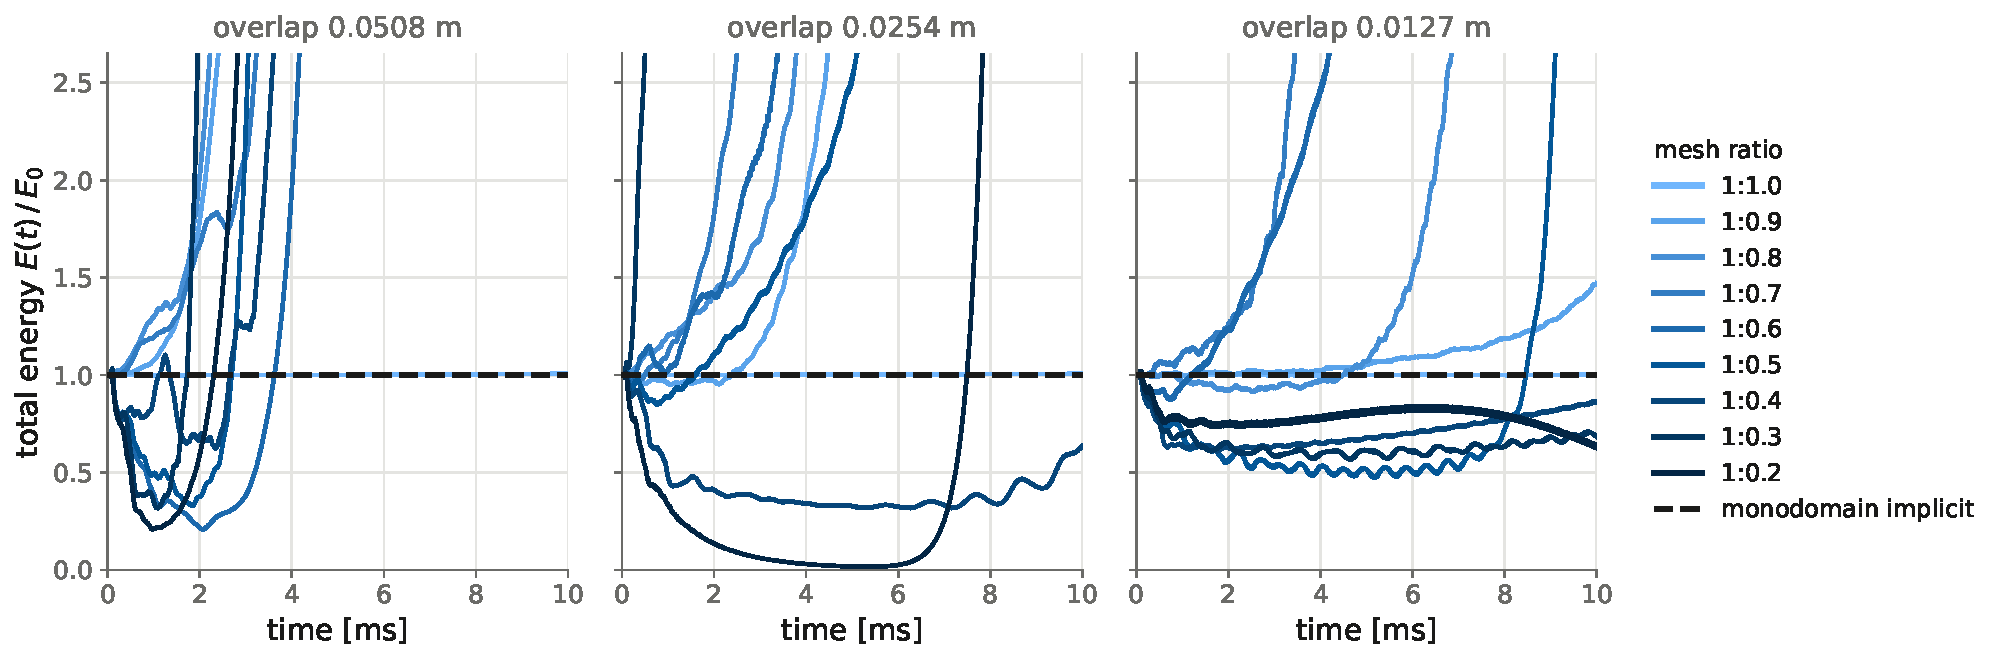
\includegraphics[width=\textwidth]{figs/overlap-II-10ms.pdf}
\caption{Overlap impedance coupling (variational transfer),
implicit--implicit, $10$\,ms. Nearly every nonconforming configuration
grows exponentially until element inversion (curves leaving the top of
the axes) or decays toward zero energy; only the conforming runs follow
the monodomain reference.}
\label{fig:overlap-10ms}
\end{figure}

\subsection{Overlap: remedies tried on the interface}
\label{sec:overlap-remedies}

Every remedy applied to the overlap exchange was measured on the
instrumented $1$\,ms benchmark; none is a structural remedy, and the
sequence explains why.

\begin{itemize}[itemsep=2pt]
\item \textbf{Transfer fidelity.} Replacing pointwise interpolation by
  the variational projection, refining the transfer quadrature, taking
  the consistent traction across the interface from the partner's offset
  surface, and transferring the whole partner datum with one operator
  each \emph{increased} the spurious dashpot work on the $1{:}0.75$ pair
  ($-607$, $-726$, $-857$, $-1129$, $-1084$\,J) while the net drift moved
  from $-0.75\%$ to $+9.8\%$: pointwise interpolation and nodal stress
  recovery had been smoothing the transferred data, and the small net of
  the original scheme was a cancellation of two large channels. Over the
  $24$ nonconforming cases of the three-ratio family the variational
  transfer improved $17$ and reduced the mean absolute drift from
  $33$ to $25\%$; it is the default because it is the contraction the
  convergence theory requires, not because it conserves.
\item \textbf{Content-aware absorption} (\code{content aware
  absorption}): an additional dissipative term
  $~W\,~Z\,(~I - \widehat\Pi)\,\dot{~u}_k$, with $\widehat\Pi$ the
  $~W$-orthogonal projection onto the transferable subspace, is verified
  (annihilates constants, vanishes on node-aligned interfaces, provably
  dissipative; test 106) and has no effect: it dissipates $4.6$\,J while
  every channel stays identical. The recirculating content lies inside
  the transferable subspace: both grids represent it, and the discrepancy
  comes from their different discrete dispersion relations, which no
  transfer construction can remove.
\item \textbf{Representable dashpot} (\code{representable dashpot}):
  restricting the dashpot to $~Z\,\widehat\Pi\,\jump{\dot{~u}}$ leaves the
  dashpot work unchanged where the projection is nontrivial
  ($-1066 \to -1065$\,J) and worsens the drift where it acts
  ($+12.5 \to +45.6\%$). Retained as a diagnostic, default off.
\item \textbf{Numerical damping.} Newmark $\gamma = 0.6$ suppresses the
  recirculation but removes $87\%$ of the physical energy. HHT-$\alpha$
  (\code{HHT alpha}, $\bar\alpha \in [0, 1/3]$) at $\bar\alpha = 0.02$ to
  $0.05$ converts the sign-indefinite drift into monotone decay with a
  loss proportional to the energy in the grid-frequency band; on this
  benchmark, whose release has content at every scale, the loss is
  $5$ to $11\%$ at $1$\,ms.
\end{itemize}

\subsection{Nonoverlap: legacy and paired coupling}
\label{sec:beam-nonoverlap}

\begin{table}[htbp]
\centering
\caption{Energy drift at 1\,ms of the nonoverlap impedance coupling on
the cantilever, in percent. Left: legacy per-side transfer against the
adjoint-paired coupling, implicit--implicit. Right: the paired coupling
in all four integrator pairings, staggered metric for explicit members.}
\label{tab:legacy-paired}
\begin{tabular}{lrr@{\hspace{2.5em}}rrrr}
\toprule
ratio & legacy II & paired II & paired II & IE & EI & EE \\
\midrule
1:1.0 & $-9.61$ & $\mathbf{-0.03}$ & $-0.03$ & $-0.11$ & $+0.20$ & $-0.27$ \\
1:0.9 & $-6.84$ & $\mathbf{-0.03}$ & $-0.03$ & $-0.10$ & $+0.29$ & $-0.27$ \\
1:0.8 & $-7.96$ & $-3.59$ & $-3.6$ & $-4.4$ & $-3.5$ & $-7.3$ \\
1:0.7 & $-2.06$ & $-6.55$ & $-6.6$ & $-6.2$ & $-5.3$ & $-9.8$ \\
1:0.6 & $-9.39$ & $-9.71$ & $-9.7$ & $-9.8$ & $-9.8$ & $-11.8$ \\
1:0.5 & $-13.25$ & $-13.32$ & $-13.3$ & $-13.8$ & $-10.2$ & $-10.5$ \\
1:0.4 & $-45.78$ & $-15.13$ & $-15.1$ & $-17.8$ & $-11.4$ & $-13.3$ \\
1:0.3 & $+18.95$ & $-15.08$ & $-15.1$ & $-11.5$ & $-26.4$ & $-20.2$ \\
1:0.2 & $+77.49$ & $-13.26$ & $-13.3$ & $-20.1$ & $-27.8$ & $-21.4$ \\
\bottomrule
\end{tabular}
\end{table}

\begin{figure}[htbp]
\centering
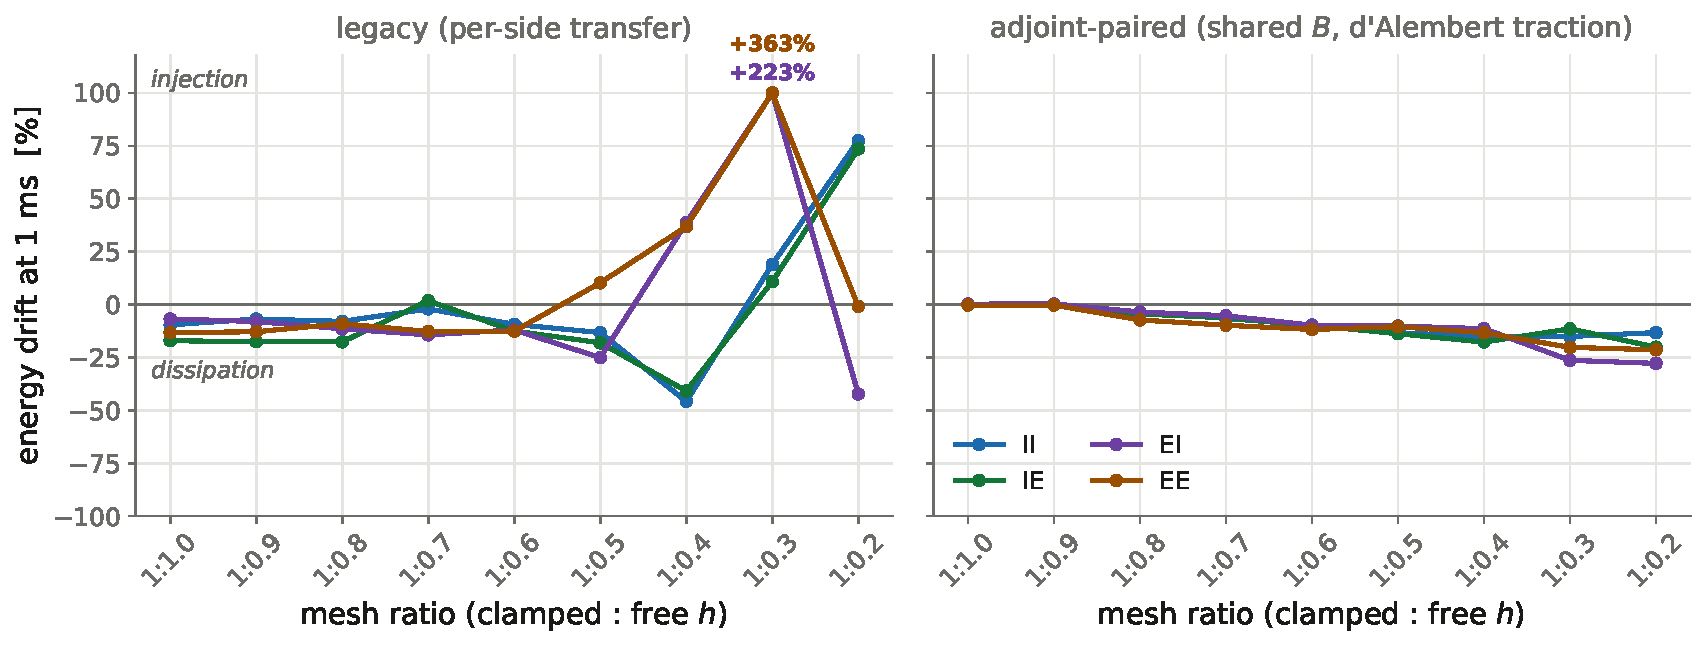
\includegraphics[width=\textwidth]{figs/legacy-vs-paired.pdf}
\caption{Nonoverlap impedance coupling, drift at 1\,ms across the
mesh-ratio family and the four integrator pairings. Left: legacy per-side
transfer (consistent-mass metric), with injection up to $+363\%$ (EE)
and $+223\%$ (EI) at $1{:}0.3$. Right: adjoint-paired coupling
(staggered metric for explicit members), sign-definite dissipation at
every ratio and conservation to $0.3\%$ on conforming and $1{:}0.9$
meshes.}
\label{fig:legacy-paired}
\end{figure}

The legacy coupling loses $2$ to $18\%$ at mild contrast in every
pairing, including on conforming meshes ($-9.6\%$ II at $1{:}1$, the
static-reaction defect of Sec.~\ref{sec:paired-construction}, unchanged
under $\alpha \to 0$, equal $\alpha$, and $\Delta t/2$), and injects
strongly at strong contrast. The paired coupling
(Table~\ref{tab:legacy-paired}, Fig.~\ref{fig:legacy-paired}) never
injects at any ratio in any pairing, conserves to $0.3\%$ on conforming
and $1{:}0.9$ meshes in all four pairings, and against the monodomain
explicit reference the conforming EE trajectory agrees to $0.35\%$
pointwise over the millisecond. The residual dissipation at strong
contrast is the interface jump the two trace spaces cannot represent in
common, absorbed at rate $Z\!\int_\Gamma \jump{\dot{~u}}^2$: at the
nested ratio $1{:}0.5$, where the legacy transfer is coincidentally
adjoint and the quadrature exact, paired and legacy agree to $0.1\%$.
The small positive EI entries are bounded transient storage in the
interface spring.

\paragraph{Ten milliseconds.} Table~\ref{tab:nonoverlap-10ms} and
Fig.~\ref{fig:nonoverlap-10ms} give the $10$\,ms behavior. With an
implicit member the conforming and $1{:}0.9$ columns stay within $0.0$ to
$-0.9\%$ over ten thousand stops. At strong contrast the dissipation that
read $10$ to $28\%$ at $1$\,ms reaches $40$ to $85\%$: bounded and
monotone, but far too large for wave-transit accuracy, since absorption
of unrepresentable content proceeds at a persistent rate. The non-nested
mild ratios $1{:}0.7$ and $1{:}0.8$ form a failure window not detectable at
$1$\,ms: interface-local high-frequency displacement content accumulates
until an interface element inverts (implicit pairs, about $5$\,ms, with
the global energy still smooth) or central difference becomes unstable
(explicit members, $2.6$ to $4$\,ms, at $0.27$ of the stability limit,
so driven by the accumulated content). Reruns with fixed $\theta = 0.5$
fail identically, so the accumulation belongs to the transfer operators,
whose partition-of-unity certificate is worst in this window; the nested
and the strong ratios do not show it.

\begin{table}[htbp]
\centering
\caption{Energy drift at 10\,ms of the adjoint-paired nonoverlap coupling
on the cantilever, staggered metric, in percent. $\dagger\,t$: element
inversion at $t$\,ms. $\ast$: bounded and noisy (Sec.~\ref{sec:energy}).}
\label{tab:nonoverlap-10ms}
\begin{tabular}{lrrrr}
\toprule
ratio & II & IE & EI & EE \\
\midrule
1:1.0 & $+0.00$ & $-0.9$ & $-0.2$ & $\ast$ \\
1:0.9 & $+0.00$ & $-0.5$ & $+0.1$ & $\ast$ \\
1:0.8 & $\dagger\,5.2$ & $\dagger\,3.9$ & $\dagger\,4.0$ & $\dagger\,2.6$ \\
1:0.7 & $\dagger\,4.9$ & $\dagger\,3.7$ & $\dagger\,3.9$ & $\dagger\,2.8$ \\
1:0.6 & $-47.3$ & $-56.4$ & $-42.9$ & $\ast$ \\
1:0.5 & $-56.8$ & $-72.0$ & $-40.8$ & $\ast$ \\
1:0.4 & $-54.9$ & $-73.9$ & $-40.4$ & $\ast$ \\
1:0.3 & $-65.1$ & $-66.0$ & $-81.1$ & $\ast$ \\
1:0.2 & $-53.3$ & $-73.1$ & $-84.1$ & $\ast$ \\
\bottomrule
\end{tabular}
\end{table}

\begin{figure}[htbp]
\centering
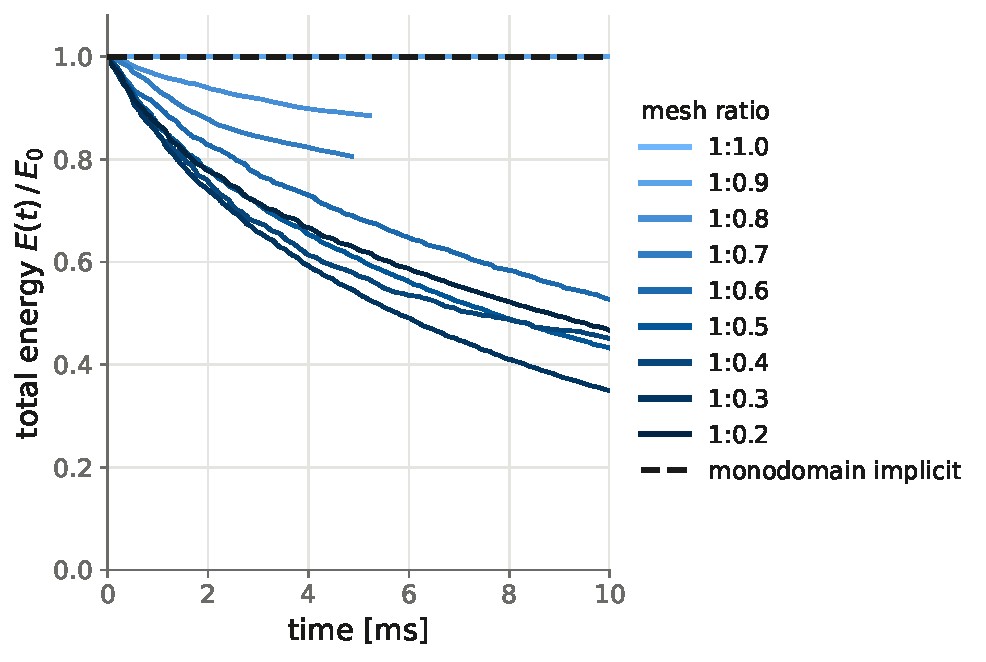
\includegraphics[width=0.495\textwidth]{figs/nonoverlap-II-10ms.pdf}\hfill
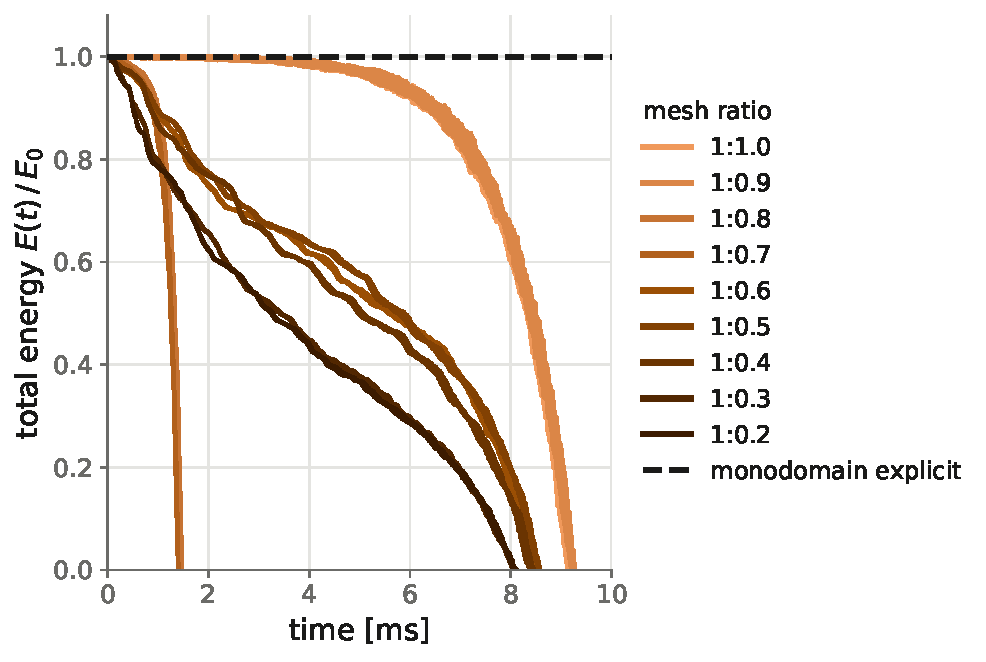
\includegraphics[width=0.495\textwidth]{figs/nonoverlap-EE-10ms.pdf}
\caption{Adjoint-paired nonoverlap coupling, $10$\,ms, staggered metric.
Left: implicit--implicit; no injection anywhere, conforming and $1{:}0.9$
follow the monodomain reference, strong contrast dissipates
monotonically, and $1{:}0.7$ to $1{:}0.8$ end at about $5$\,ms by element
inversion. Right: explicit--explicit; the staggered kinetic term goes
negative at every ratio as undamped grid-frequency content accumulates,
and $1{:}0.7$ to $1{:}0.8$ fail by central-difference instability at
$2.6$ to $2.8$\,ms.}
\label{fig:nonoverlap-10ms}
\end{figure}

\paragraph{Explicit--explicit pairs.} The EE column ends bounded and
noisy at every ratio, conforming included: the stored energy stays
physical (the conforming run keeps $E/E(0) \ge 0.97$ to $5$\,ms) while
the staggered kinetic term goes negative, because central difference with
$\gamma = \tfrac12$ removes no grid-frequency content at any stable step
and the exchange keeps introducing it. Subcycling the explicit member
(free side at $\Delta t/4$) removes the accumulation: that run ends at
$-10.8\%$, the dissipation of the interpolated exchange. Subcycling has
the opposite effect on implicit pairs, where the same-step conforming II
run conserves to $0.00\%$ and the subcycled one loses $-20.2\%$ over
$10^4$ stops ($-3.6\%$ at $1$\,ms), the interpolation dissipation of
Sec.~\ref{sec:subcycle} accumulated over the run.

\subsection{Windowed controller stops}
\label{sec:windowed}

With the subdomain steps fixed at $1\,\mu$s, controller stops of $1$,
$2$, $5$, and $10\,\mu$s were compared to $10$\,ms. For the overlap
family every trajectory is identical across the four windows (its
exchange has no relaxation state). For the nonoverlap coupling the
pre-fix per-pair relaxation state shifted the fixed point
(Sec.~\ref{sec:relaxation}); with the slot-keyed state every windowed
policy reproduces the same-step trajectory to Schwarz truncation (a
displacement mismatch of $3.9\times 10^{-6}$ at working tolerances,
$3.7\times 10^{-8}$ at tightened ones; regression in test 110). Inside a
window the policies were measured on the conforming II case at the
$10\,\mu$s window, in mean Schwarz iterations per stop: $\theta = 1$
needs $19.1$ and completes; per-slot Aitken about $25$ and fails at
$3.9$\,ms; fixed $\theta = 0.5$ $47.5$; Aitken pooled over the window's
slots $55.1$ on II and fails on EE. The total number of substep solves
is proportional to the iterations per stop whatever the window, and all
windowed counts exceed the same-step Aitken count, so the controller
step is a convenience for the nonoverlap coupling (for aligning output
stops) and never reduces work; for the overlap family larger stops
reduce it slightly. The explicit--explicit pair at large windows is
impractical under any policy (the windowed iteration is nearly
non-contractive and reaches the iteration cap).

\subsection{The five couplings with the current code}
\label{sec:beam-five}

The five couplings (overlap Dirichlet, nonoverlap Dirichlet--Neumann,
overlap impedance, paired nonoverlap impedance, and the monolithic
reference) were rerun to $10$\,ms with the code of 2026-09-17 at ratios
$1{:}0.9$, $1{:}0.75$, and $1{:}0.5$ with overlap $25.4$\,mm
(Table~\ref{tab:beam-five}, Fig.~\ref{fig:beam-five}). The
Dirichlet--Neumann exchange, not part of the earlier study, ends by
element inversion within $3$\,ms with implicit subdomains at every ratio
and conserves within $1\%$ to $10$\,ms with explicit ones; why the same
exchange is unstable with implicit subdomains and stable with explicit
ones has not been explained (Sec.~\ref{sec:open}). Every other entry
reproduces the corresponding earlier result.

\begin{table}[htbp]
\centering
\footnotesize\setlength{\tabcolsep}{3.5pt}
\caption{Cantilever, overlap 25.4\,mm, code of 2026-09-17:
$E(10\,\mathrm{ms})/E(0)$, or the time the run ended by element
inversion. ``Bounded, noisy'' is the explicit state of
Sec.~\ref{sec:energy}.}
\label{tab:beam-five}
\begin{tabular}{lcccccc}
\toprule
coupling & 1:0.9 II & 1:0.9 EE & 1:0.75 II & 1:0.75 EE & 1:0.5 II & 1:0.5 EE \\
\midrule
monolithic & 1.000 & 1.000 & 1.000 & 1.000 & 1.000 & 1.000 \\
overlap, Dirichlet & 3.16 & fails 4.9\,ms & fails 1.5\,ms & fails 2.1\,ms & fails 0.9\,ms & fails 1.3\,ms \\
nonoverlap, Dirichlet--Neumann & fails 2.9\,ms & 1.006 & fails 0.4\,ms & 1.002 & fails 0.7\,ms & 1.008 \\
overlap, impedance & fails 7.2\,ms & fails 8.4\,ms & fails 6.0\,ms & 12.2 & fails 7.3\,ms & 5.9 \\
nonoverlap, impedance (paired) & 1.000 & bounded, noisy & fails 5.0\,ms & fails 2.6\,ms & 0.43 & bounded, noisy \\
\bottomrule
\end{tabular}
\end{table}

\begin{figure}[htbp]
\centering
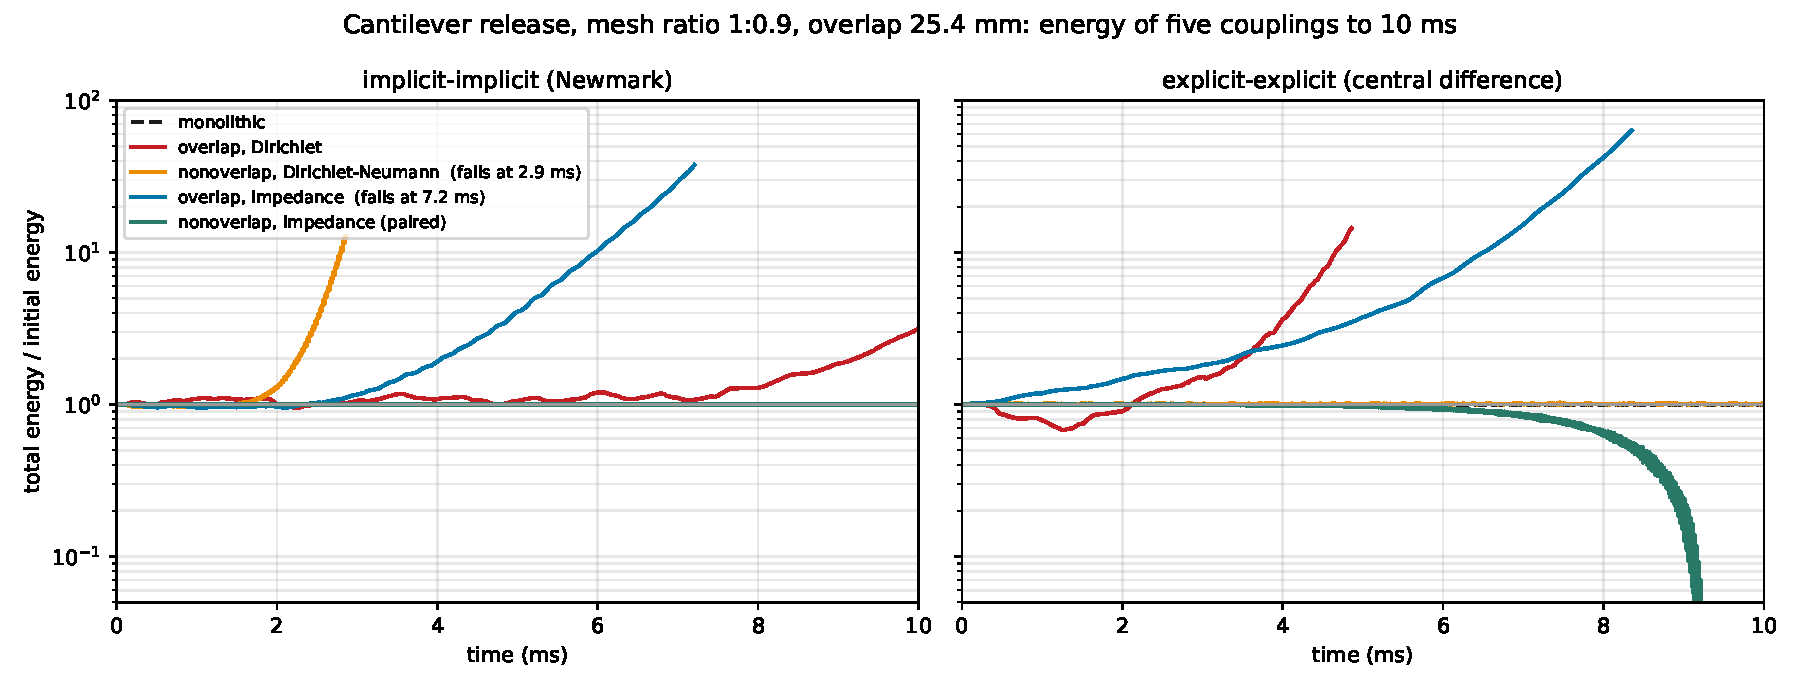
\includegraphics[width=\textwidth]{figs/beam-five-couplings.pdf}
\caption{Cantilever at mesh ratio $1{:}0.9$, overlap $25.4$\,mm, five
couplings to $10$\,ms, code of 2026-09-17. Left: implicit--implicit.
Right: explicit--explicit; the paired impedance curve ends in the
bounded, noisy state.}
\label{fig:beam-five}
\end{figure}

\subsection{The classical Robin--Robin condition}
\label{sec:beam-rr}

The Robin--Robin condition was run on both decompositions on 2026-09-18:
\code{Schwarz RR nonoverlap} with the classical per-side transfer, and
\code{Schwarz impedance overlap} with \code{impedance scale: 0}. Since
the converged solution and the iteration both depend on $\alpha$ on
nonconforming meshes, two values, one near the Dirichlet limit and one near the
Neumann limit, were used: $\alpha = E/h = 10^{12}$\,N/m$^3$
with $h = 6.35$\,mm, and $\alpha = E/L = 2.7\times 10^{10}$\,N/m$^3$ with
$L = 254$\,mm. Integrators, ratios, relaxation, and tolerances are those
of Table~\ref{tab:beam-five}. Every run converged in $2$ to $4$ Schwarz
iterations per stop, so Table~\ref{tab:beam-rr} shows the converged
coupling.

\begin{table}[htbp]
\centering
\footnotesize\setlength{\tabcolsep}{3.5pt}
\caption{Cantilever, classical Robin--Robin coupling, overlap 25.4\,mm:
$E(10\,\mathrm{ms})/E(0)$, or the time the run ended by element
inversion.}
\label{tab:beam-rr}
\begin{tabular}{lcccccc}
\toprule
coupling & 1:0.9 II & 1:0.9 EE & 1:0.75 II & 1:0.75 EE & 1:0.5 II & 1:0.5 EE \\
\midrule
overlap, $\alpha = E/h$ & fails 0.7\,ms & fails 1.4\,ms & fails 0.8\,ms & fails 1.9\,ms & fails 0.4\,ms & fails 0.8\,ms \\
overlap, $\alpha = E/L$ & fails 0.9\,ms & fails 1.1\,ms & fails 0.9\,ms & fails 1.5\,ms & fails 1.6\,ms & fails 5.4\,ms \\
nonoverlap, $\alpha = E/h$ & fails 1.2\,ms & fails 2.4\,ms & fails 1.1\,ms & fails 0.2\,ms & fails 0.3\,ms & fails 0.3\,ms \\
nonoverlap, $\alpha = E/L$ & fails 7.1\,ms & 0.96 (peak 1.05) & fails 7.4\,ms & fails 4.5\,ms & fails 3.4\,ms & fails 0.9\,ms \\
\bottomrule
\end{tabular}
\end{table}

\begin{figure}[htbp]
\centering
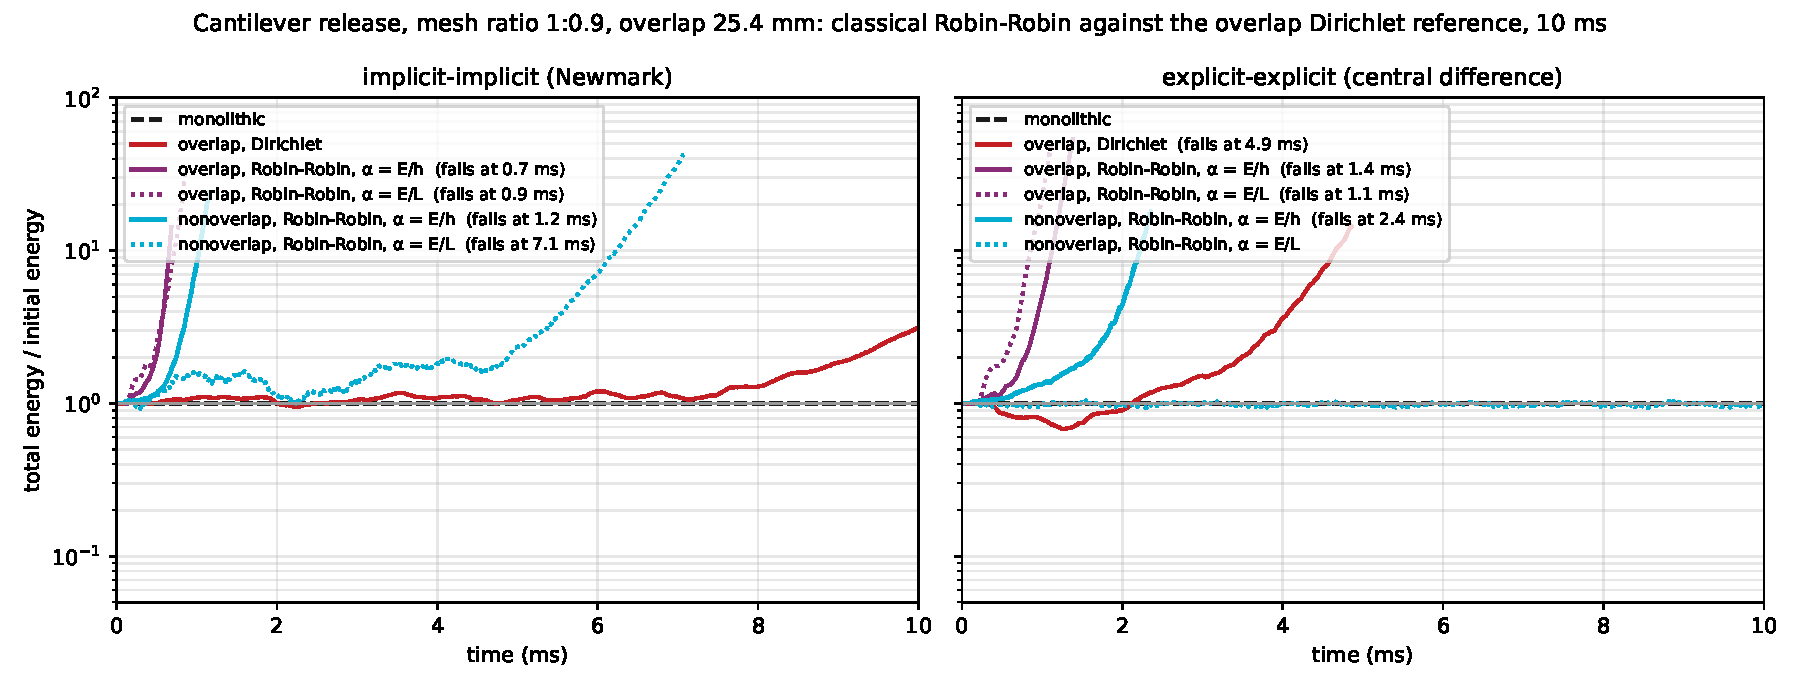
\includegraphics[width=\textwidth]{figs/beam-robin-robin.pdf}
\caption{Cantilever at mesh ratio $1{:}0.9$: classical Robin--Robin
coupling on both decompositions at two Robin parameters, against the
overlap Dirichlet reference, $10$\,ms.}
\label{fig:beam-rr}
\end{figure}

Twenty-three of the $24$ runs end by element inversion after exponential
growth, between $0.2$ and $7.4$\,ms; the one survivor ($1{:}0.9$, EE,
$\alpha = E/L$) stays within $5\%$ to $10$\,ms. The growth is faster than
with overlap Dirichlet transmission in $18$ of the $24$ cases, and the
stiffer spring fails sooner in $10$ of the $12$ pairs. The converged
coupled solution depends on $\alpha$ (the two nonoverlap rows differ
although both are converged to $10^{-8}$): with per-side transfer on
nonconforming meshes the discrete jump does not close, and the spring
force on the residual jump scales with $\alpha$. The result is the one
\eqref{eq:R-rr} predicts: a condition that reflects every wave has no
term that damps the interface mode fed by the discrete mismatch, and
the spring stores that mismatch. The dashpot of the impedance condition
is the term that removes it.

\section{Measurements on the nested cylinders}
\label{sec:cylinders}

The cylinders (Sec.~\ref{sec:benchmark}) were built as a second case that
excites the instability independently of the beam: three materials with a
fiftyfold impedance contrast, a compressive front instead of flexure, and
a closed curved interface with caps, at a mild mesh ratio ($1{:}0.8$).
Every subdomain is explicit. The Schwarz iteration uses Aitken
relaxation for the Dirichlet--Neumann exchange, a fixed factor
$\theta = 0.5$ for the paired impedance and Robin--Robin couplings
(Sec.~\ref{sec:relaxation}), and no relaxation for the overlap couplings,
with a relative tolerance of $10^{-6}$ and an absolute tolerance of
$10^{-4}$. The monolithic
reference conserves the blended staggered energy to $0.01\%$ over the
$10^4$ steps. Table~\ref{tab:cylinders} and
Figs.~\ref{fig:cylinders}--\ref{fig:cylinders-rr} give the results.

\begin{table}[htbp]
\centering
\small
\caption{Nested cylinders, explicit on both sides, $5$\,ms:
$E(t)/E(0)$ at the times shown, or the time the run ended by element
inversion. Robin--Robin at $\alpha = E/h = 3.4\times 10^{10}$ and
$\alpha = E/L = 2.8\times 10^{9}$\,N/m$^3$, with $E$ the Young's modulus
of the filler, $h = 6.35$\,mm, and $L = 76$\,mm.}
\label{tab:cylinders}
\begin{tabular}{lcccc}
\toprule
coupling & 0.5\,ms & 1\,ms & 2\,ms & 5\,ms \\
\midrule
overlap, Dirichlet & 1.02 & 1.29 & \multicolumn{2}{l}{fails 1.54\,ms at $7.4\,E(0)$} \\
overlap, impedance & 1.02 & 1.76 & \multicolumn{2}{l}{fails 1.26\,ms at $13\,E(0)$} \\
overlap, Robin--Robin, $\alpha = E/h$ & 1.63 & \multicolumn{3}{l}{fails 0.66\,ms at $5.5\,E(0)$} \\
overlap, Robin--Robin, $\alpha = E/L$ & 1.53 & \multicolumn{3}{l}{fails 0.75\,ms at $11\,E(0)$} \\
nonoverlap, Dirichlet--Neumann & 1.00 & 1.00 & 1.01 & 1.00 \\
nonoverlap, Robin--Robin, $\alpha = E/h$ & 1.27 & \multicolumn{3}{l}{fails 0.81\,ms at $3.1\,E(0)$} \\
nonoverlap, Robin--Robin, $\alpha = E/L$ & 1.08 & 1.26 & 2.45 & fails 3.59\,ms at $11\,E(0)$ \\
nonoverlap, impedance (paired), 2 iterations per stop & 0.79 & 0.54 & 0.24 & 0.065 \\
same, 6 iterations per stop (to 1\,ms) & 0.89 & 0.77 & --- & --- \\
same, $\theta = 1$ & \multicolumn{4}{l}{0.997 to 0.3\,ms, then the iteration diverges} \\
\bottomrule
\end{tabular}
\end{table}

\begin{figure}[htbp]
\centering
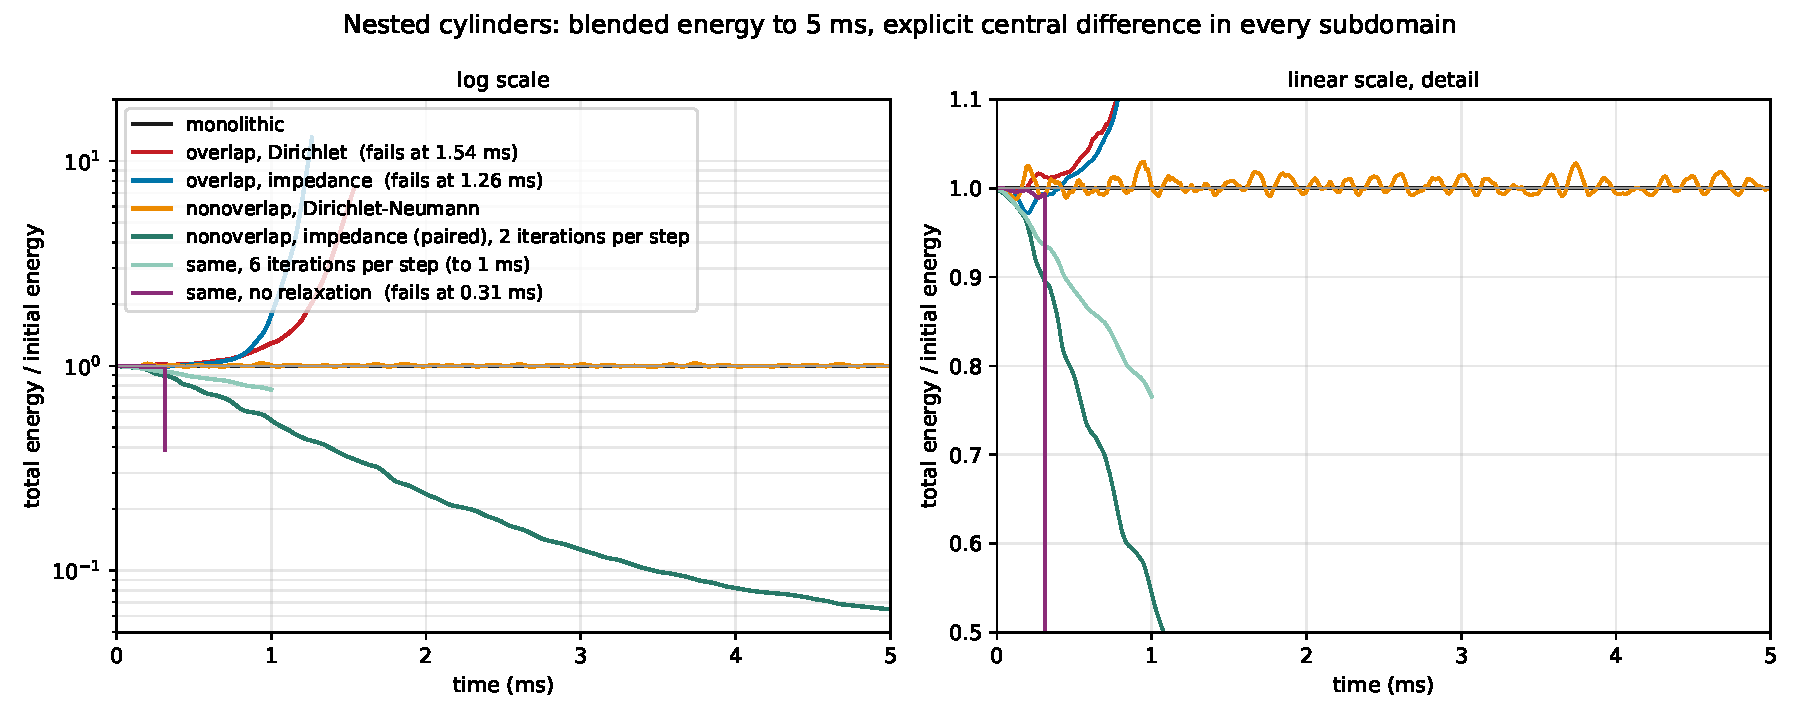
\includegraphics[width=\textwidth]{figs/cylinders-couplings.pdf}
\caption{Nested cylinders, blended staggered energy to $5$\,ms: the
Dirichlet and impedance couplings on both decompositions, with the two
diagnostic variants of the paired coupling.}
\label{fig:cylinders}
\end{figure}

\begin{figure}[htbp]
\centering
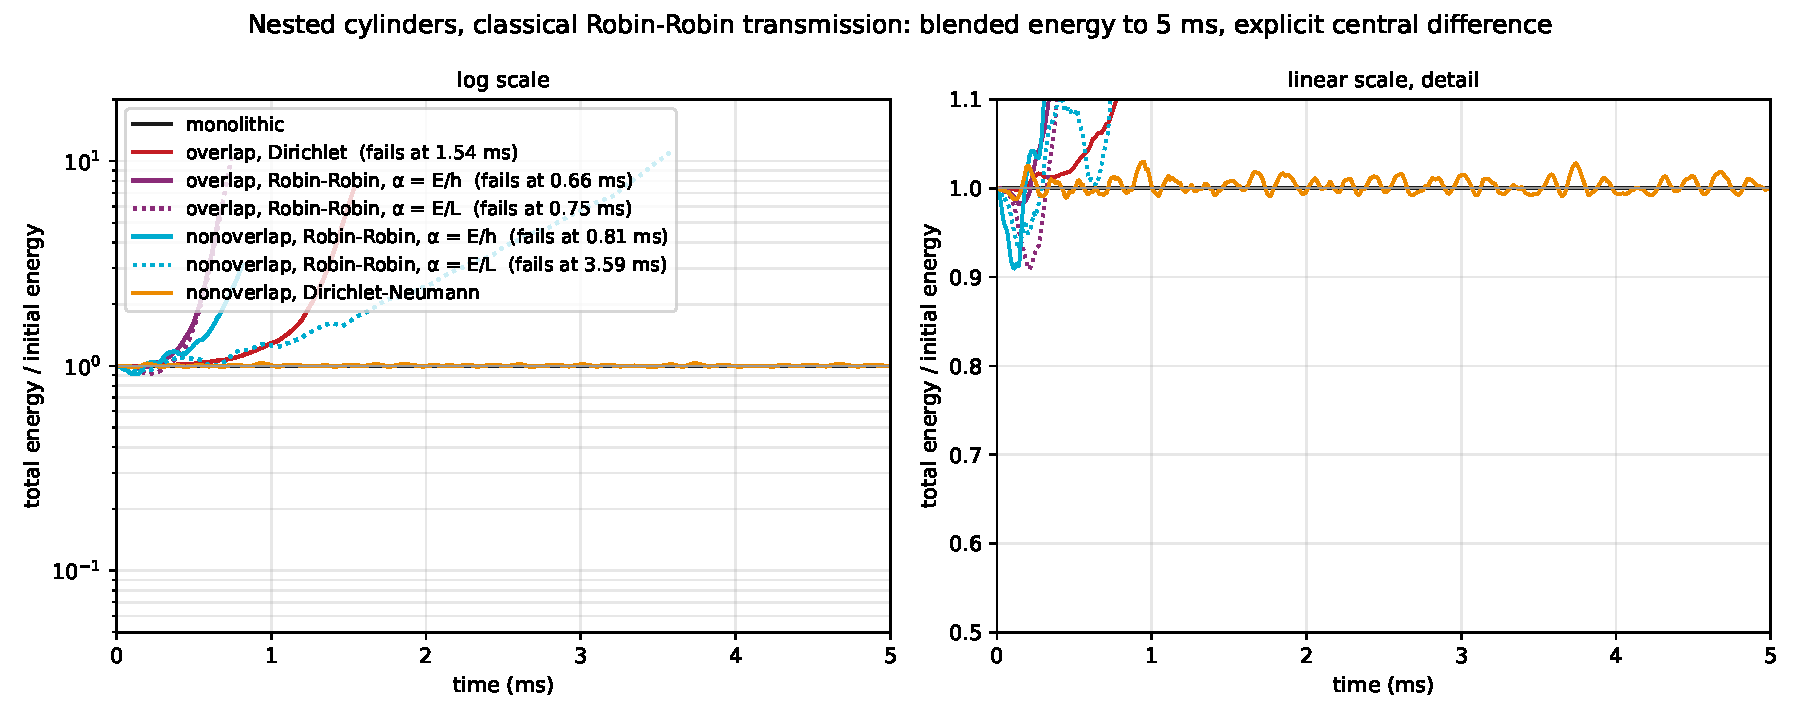
\includegraphics[width=\textwidth]{figs/cylinders-robin-robin.pdf}
\caption{Nested cylinders, classical Robin--Robin coupling on both
decompositions at two Robin parameters, against the overlap Dirichlet
and nonoverlap Dirichlet--Neumann references.}
\label{fig:cylinders-rr}
\end{figure}

\paragraph{Dirichlet couplings.} Overlap Dirichlet coupling leaves the
reference after $0.4$\,ms, grows exponentially, and ends by element
inversion at $1.54$\,ms at $7.4\,E(0)$: the same mechanism and a
comparable rate as on the beam, although the interface here is closed
and the meshes only mildly nonconforming. The nonoverlap
Dirichlet--Neumann exchange (Aitken relaxation, $2$ iterations per stop)
stays within $+3$ and $-1.3\%$ for the whole $5$\,ms, as on the beam with
explicit subdomains.

\paragraph{Impedance couplings.} Overlap impedance coupling is unstable
and faster than Dirichlet: it reaches $13\,E(0)$ at $1.26$\,ms. On the
beam the same condition survived $6$ to $8$\,ms; here the dashpot faces
the inter-grid discrepancy of a compressive front resolved with $5$ and
$6$\,mm elements. The paired nonoverlap coupling never grows but
dissipates strongly: $0.54\,E(0)$ at $1$\,ms and $0.065$ at $5$\,ms.
The interface velocity jump stalls at $0.1$ to $0.14$ of its initial size
at every stop and is accepted by the displacement criterion, so the
dashpot keeps absorbing it. Six iterations per stop keep $0.77\,E(0)$ at
$1$\,ms instead of $0.54$, so about half of the loss is iteration lag on
a jump the criterion does not measure; no relaxation keeps $0.997\,E(0)$ to
$0.3$\,ms and then fails to converge within $256$ iterations. Every
Aitken form diverges on this pair (Sec.~\ref{sec:relaxation}).

\paragraph{Robin--Robin.} All four runs end by element inversion after
exponential growth. The overlap runs fail sooner than overlap Dirichlet
($1.54$\,ms) and overlap impedance ($1.26$\,ms); the nonoverlap runs fail
where the paired impedance coupling never grows and the
Dirichlet--Neumann exchange holds. The Schwarz iteration converged in
$1$ to $2$ iterations per stop. As on the beam, the stiffer spring fails
sooner, and the softer nonoverlap spring lasts longest, $3.6$\,ms, still
growing to $11\,E(0)$.

\section{Conclusions}
\label{sec:conclusion}

\subsection{Findings}

\begin{enumerate}[itemsep=2pt]
\item Dirichlet transmission on nonconforming meshes injects energy on
  both benchmarks, on the overlap decomposition and on the implicit
  nonoverlap Dirichlet--Neumann exchange: exponential growth ending in
  element inversion, at comparable rates on a flexural beam and on a
  shock-loaded nested assembly (Secs.~\ref{sec:overlap-nonconforming},
  \ref{sec:beam-five}, \ref{sec:cylinders}).
\item The classical Robin--Robin condition is not a remedy. It reflects
  every wave ($\lvert R \rvert \equiv 1$), has no term that damps the
  interface mode, and pumps energy on both benchmarks and both
  decompositions, usually faster than Dirichlet transmission, at either
  Robin parameter; with per-side transfer its converged solution depends
  on $\alpha$ (Secs.~\ref{sec:beam-rr}, \ref{sec:cylinders}).
\item On an overlap boundary the impedance condition is consistent with
  the monodomain solution only with the partner traction, and with the
  consistent traction it is exact on conforming meshes ($0.08\%$ at
  $1$\,ms, no parameters). On nonconforming meshes its interface work is
  sign-indefinite in principle (two surfaces, non-adjoint transfers) and
  in practice (injection up to $+275\%$, sign changes between adjacent
  ratios, $74$ of $108$ runs failing by $10$\,ms), and no construction at
  the interface changes that, because the discrepancy is the difference
  of the two grids' dispersion relations, which both grids represent
  (Secs.~\ref{sec:conforming}--\ref{sec:overlap-remedies}). On the
  cylinders it fails sooner than Dirichlet coupling.
\item Energy consistency requires one interface traction acting through
  adjoint transfers built from one cross-mass matrix; the interface power
  is then the sign-definite dissipation \eqref{eq:telescope} on the
  interface jump. Only the nonoverlap decomposition, with its shared
  interface, admits this construction (Sec.~\ref{sec:theory}).
\item The adjoint-paired nonoverlap coupling never injects energy at any
  ratio, pairing, or benchmark. On the beam it conserves to $0.3\%$ at
  $1$\,ms and to $0.0\%$ at $10$\,ms on conforming and $1{:}0.9$ meshes
  with an implicit member; at strong contrast it dissipates the
  unrepresentable jump at a persistent rate ($40$ to $85\%$ by $10$\,ms);
  the non-nested ratios $1{:}0.7$ to $1{:}0.8$ accumulate interface-local
  high-frequency content until an element inverts at $3$ to $5$\,ms; and
  explicit--explicit pairs end bounded but noisy, which subcycling the
  explicit member removes (Sec.~\ref{sec:beam-nonoverlap}).
\item On the cylinders the paired coupling is stable but loses half the
  energy within $1$\,ms, because the iteration stops on displacement
  while the interface velocity jump, which the dashpot damps, stalls at a
  finite value; more iterations halve the loss, and no relaxation nearly
  removes it before the iteration diverges (Sec.~\ref{sec:cylinders}).
\item Different time steps per subdomain use piecewise-linear
  interpolation of the partner trajectory, whose dissipation of order
  $\Delta t$ is the energy loss intrinsic to subcycling; exact
  cancellation of the subcycled interface work is incompatible with a
  partitioned exchange (Sec.~\ref{sec:subcycle}).
\item The relaxation state must be keyed per pair and per substep slot;
  Aitken acceleration applies to single-slot stops only, reduces the
  iteration count tenfold on the implicit beam pairs, and diverges in every form on
  the explicit cylinders pair, where a fixed factor of $0.5$ converges in
  $2$ to $3$ iterations (Sec.~\ref{sec:relaxation}).
\item With explicit subdomains on both sides the plain
  Dirichlet--Neumann exchange conserved on both benchmarks (within $1\%$
  on the beam, $3\%$ on the cylinders), while with implicit subdomains it
  is the fastest coupling to fail.
\end{enumerate}

\subsection{Recommendations}

\begin{itemize}[itemsep=2pt]
\item \textbf{Energy-critical dynamic coupling}: use the adjoint-paired
  nonoverlap impedance coupling (the default of \code{Schwarz impedance
  nonoverlap}) with at least one implicit interface member and a
  conforming or nested mesh ratio; avoid non-nested mild ratios for long
  runs. Use a fixed relaxation factor with explicit pairs, Aitken with
  implicit ones.
\item \textbf{Overlap decompositions}: conforming meshes with
  implicit--implicit integration conserve at any horizon; every other
  overlap configuration is for short transients only.
\item \textbf{Robin--Robin}: for quasi-statics and comparison studies
  only.
\item \textbf{All-explicit interfaces}: subcycle the finer side, or
  accept the bounded, noisy state; central difference removes no
  grid-frequency content at any stable step.
\item \textbf{Parameters}: the impedance is material data (harmonic mean
  per pair for nonoverlap, partner material with P/S split for overlap);
  no scaling. The Robin parameter must be one value per interface under
  pairing and affects only the iteration when the jump can close; on
  nonconforming meshes its effect on the converged solution is
  unmeasured for the paired coupling, and the runs in this note use
  $\alpha = 0$ or $2\times 10^{9}$\,N/m$^3$.
\item \textbf{Diagnostics}: use the blended energy output with the
  staggered metric for explicit members, and the channel-resolved
  interface-work instrumentation as the acceptance metric for any change
  to the transmission machinery; a small net drift can be the difference
  of two large channels.
\end{itemize}

\subsection{Open questions}
\label{sec:open}

\begin{enumerate}[label=(\roman*),itemsep=2pt]
\item The stalled interface jump on the cylinders: a stopping criterion
  that refuses a stalled velocity jump, relaxation factors between $0.5$
  and $1$, and subcycling of the explicit side are the candidates for
  recovering the energy the paired coupling now dissipates.
\item The dependence of the converged paired solution on $\alpha$ and on
  $\theta$: the fixed point differs by about $4\times 10^{-5}$ relative
  displacement between $\theta = 0.5$ and $1$ at a $10^{-13}$ tolerance
  on the $1{:}0.5$ beam, evidence of a neutral mode of the exchange that
  the displacement criterion does not measure; an $\alpha$ sweep of the
  paired coupling on nonconforming meshes has not been run.
\item Why the Dirichlet--Neumann exchange is stable between explicit
  subdomains and unstable between implicit ones.
\item The non-nested mesh-ratio failure window of the paired transfer at
  long horizons.
\item Exact subcycled interface-work cancellation through a direct
  interface solve, with the localized Lagrange multiplier frame
  construction~\cite{ParkFelippaRebel2002,DvorakEtAl2023}.
\item Mesh-ratio and overlap-width families on the cylinders, and
  implicit versions of its subdomains, to test whether the beam
  conclusions transfer.
\end{enumerate}

\subsection*{Data provenance}

Correction-sequence study and instrumentation:
\path{rigel:~/test/Norma/cantilever-energy}. Mesh-ratio sweep,
$10$\,ms horizon, controller-step sweep, and run harness:
\path{sirius:~/cantilever-energy-study/}. The 2026-09 reruns,
the Robin--Robin runs, and the cylinders runs:
\path{rigel:~/test/Norma/beam/} (\code{runs}, \code{runs-r090},
\code{runs-r050}) and \path{rigel:~/test/Norma/cylinders/}. Slides:
\path{Norma-Energy-Stability-Beam-Cylinders-2026-09.pptx}. Regression
tests: 104 (overlap impedance energy and consistent-traction patch), 105
(tensor impedance cross-scaling), 106 (variational transfer projectors
and content-absorption dissipativity), 110 (adjoint pairing, windowed
equivalence, keyword guards), 125 (explicit stable step with
subcycling).
\begin{thebibliography}{99}

\bibitem{MotaTezaurPhlipot2022}
A.~Mota, I.~Tezaur, G.~Phlipot,
The Schwarz alternating method for transient solid dynamics,
\emph{International Journal for Numerical Methods in Engineering}
123:5036--5071, 2022.

\bibitem{MotaKoliesnikovaTezaurHoy2023}
A.~Mota, D.~Koliesnikova, I.~Tezaur, J.~Hoy,
A fundamentally new coupled approach to contact mechanics via the
Dirichlet--Neumann Schwarz alternating method,
arXiv:2311.05643, 2023.

\bibitem{LysmerKuhlemeyer1969}
J.~Lysmer, R.L.~Kuhlemeyer,
Finite dynamic model for infinite media,
\emph{Journal of the Engineering Mechanics Division (ASCE)}
95(EM4):859--877, 1969.

\bibitem{GravouilCombescure2001}
A.~Gravouil, A.~Combescure,
Multi-time-step explicit--implicit method for non-linear structural
dynamics,
\emph{International Journal for Numerical Methods in Engineering}
50:199--225, 2001.

\bibitem{PrakashHjelmstad2004}
A.~Prakash, K.D.~Hjelmstad,
A FETI-based multi-time-step coupling method for Newmark schemes in
structural dynamics,
\emph{International Journal for Numerical Methods in Engineering}
61:2183--2204, 2004.

\bibitem{KarimiNakshatrala2014}
S.~Karimi, K.B.~Nakshatrala,
On multi-time-step monolithic coupling algorithms for elastodynamics,
\emph{Journal of Computational Physics} 273:671--705, 2014.

\bibitem{GanderHalpernNataf2003}
M.J.~Gander, L.~Halpern, F.~Nataf,
Optimal Schwarz waveform relaxation for the one dimensional wave equation,
\emph{SIAM Journal on Numerical Analysis} 41(5):1643--1681, 2003.

\bibitem{AchdouJaphetMadayNataf2002}
Y.~Achdou, C.~Japhet, Y.~Maday, F.~Nataf,
A new cement to glue non-conforming grids with Robin interface conditions:
the finite volume case,
\emph{Numerische Mathematik} 92(4):593--620, 2002.

\bibitem{AppeloWang2019}
D.~Appel\"o, S.~Wang,
An energy-based discontinuous Galerkin method for coupled elasto-acoustic
wave equations in second-order form,
\emph{International Journal for Numerical Methods in Engineering}
119(7):618--638, 2019.

\bibitem{DuruEtAl2021}
K.~Duru, L.~Rannabauer, A.-A.~Gabriel, O.K.A.~Ling, H.~Igel, M.~Bader,
A stable discontinuous Galerkin method for linear elastodynamics in 3D
geometrically complex elastic solids using physics based numerical fluxes,
arXiv:1907.02658, 2021.

\bibitem{LiuEtAl2023}
Q.Q.~Liu, M.~Zhuang, W.~Zhan, L.~Shi, Q.H.~Liu,
A hybrid implicit--explicit discontinuous Galerkin spectral element time
domain (DG-SETD) method for computational elastodynamics,
\emph{Geophysical Journal International} 234:1855--1869, 2023.

\bibitem{ParkFelippaRebel2002}
K.C.~Park, C.A.~Felippa, G.~Rebel,
A simple algorithm for localized construction of non-matching structural
interfaces,
\emph{International Journal for Numerical Methods in Engineering}
53:2117--2142, 2002.

\bibitem{DvorakEtAl2023}
R.~Dvo\v{r}\'ak, R.~Kolman, M.~Mra\v{c}ko, J.~Kopa\v{c}ka, T.~F\'ila,
O.~Jirou\v{s}ek, J.~Falta, M.~Neuh\"auserov\'a, V.~Rada, V.~Ad\'amek,
J.A.~Gonz\'alez,
Energy-conserving interface dynamics with asynchronous direct time
integration employing arbitrary time steps,
\emph{Computer Methods in Applied Mechanics and Engineering} 413:116110,
2023.

\end{thebibliography}

\end{document}
